%%====================%%
%%  Part III Project  %%
%%====================%%
% 1. Save the original kernel definition
\let\latexaddtocontents\addtocontents

\documentclass[aps,prd,reprint,preprintnumbers,showpacs,floatfix,nofootinbib,superscript address]{revtex4-2}
\usepackage[utf8]{inputenc}
\usepackage{parskip}
\usepackage{amssymb}
\usepackage{stix}
\usepackage{hhline}
\usepackage{amsmath}
\usepackage{amsfonts}
\usepackage{mathtools}
\usepackage{amsmath}
\usepackage[dvipsnames]{xcolor}
\usepackage{xspace}
\usepackage{multirow,tabularx}
\usepackage{siunitx}
\usepackage{multirow}
\usepackage{graphicx}
\usepackage{xstring}
\usepackage{etoolbox}
\usepackage{notoccite}
\usepackage{mathrsfs}
\usepackage{lineno}
\usepackage{tensor}
\usepackage{stackengine,scalerel}
\usepackage{accents}
\usepackage{tikz}
\usepackage{listings}
\usepackage{bm}
\usepackage{comment}
\allowdisplaybreaks
\parskip 1mm
\parindent 2mm

%%===========================%%
%%  Part III Project Macros  %%
%%===========================%%

%	The Planck mass
\newrobustcmd{\Planck}{%
	{M_{\text{Pl}}}%
}

%	The Riemannian covariant derivative
\newrobustcmd{\rD}[1]{%
	\tensor{\mathring{\nabla}}{#1}%
}

%	The Riemann-Cartan covariant derivative
\newrobustcmd{\rcD}[1]{%
	\tensor{\nabla}{#1}%
}

%	The Riemann tensor
\newrobustcmd{\rR}[1]{%
	\tensor{\mathring{R}}{#1}%
}

%	The Riemann-Cartan tensor
\newrobustcmd{\rcR}[1]{%
	\tensor{R}{#1}%
}

%	Irreducible parts of the torsion
\newrobustcmd{\T}[2][placeholder]{%
	\IfEqCase{#1}{%
	{placeholder}{\tensor{T}{#2}}%
	{1}{\tensor[^{(1)}]{T}{#2}}%
	{2}{\tensor[^{(2)}]{T}{#2}}%
	{3}{\tensor[^{(3)}]{T}{#2}}%
	}%
	[\packageError{cosmicclass}{Symbol #1 is not an irreducible part!}{}]%
}

%	Irreducible parts of the multiplier
\newrobustcmd{\TLambda}[2][placeholder]{%
	\IfEqCase{#1}{%
	{placeholder}{\tensor{\lambda}{#2}}%
	{1}{\tensor[^{(1)}]{\lambda}{#2}}%
	{2}{\tensor[^{(2)}]{\lambda}{#2}}%
	{3}{\tensor[^{(3)}]{\lambda}{#2}}%
	}%
	[\packageError{cosmicclass}{Symbol #1 is not an irreducible part!}{}]%
}
 %some personal macros

\usepackage{hyperref}
\hypersetup{%
     colorlinks = true,%
     linkcolor = Blue,%
     citecolor = Blue,%
     filecolor = Blue,%
     urlcolor = Blue,%
     pdftitle={Master's Thesis - Prabhoda Chandra Sarjapur},%
    pdfpagemode=FullScreen,%
     }%
\newcommand{\signature}[2][8em]{%
  \begin{tabular}[t]{ p{#1} p{#1} }
    \strut\raggedleft
    \raisebox{-.5ex}[0pt][0pt]{\bfseries #2} & \\
    \cline{2-2}
    & \centering\scriptsize\itshape (signature)
  \end{tabular}
}


\makeatletter
  \let\addtocontents\latexaddtocontents
\makeatother

% 4. Now load biblatex as usual
\usepackage[backend=biber,style=vancouver]{biblatex}

\usepackage[style=nejm, 
citestyle=numeric-comp,
sorting=none]{biblatex}
\addbibresource{Bibliography.bib}


\nocite{*}

\newcommand{\wb}[1]{{\color[RGB]{255,0,0}{\textbf{\textit{[WB: #1]}}}}}
\newcommand{\pcs}[1]{{\color[RGB]{0,100,0}{\textbf{\textit{[PCS: #1]}}}}}

\usepackage{titlesec}
\newrobustcmd{\pea}[1]{\emph{#1}\textbf{.\ \ \ ---}}
\titleformat{\paragraph}[runin]{\normalfont\normalsize\bfseries}{\emph\theparagraph}{1em}{\pea}
\titleformat{\section}[block]{\normalfont\bfseries\centering}{\MakeUppercase\thesection}{1em}{\MakeUppercase}
\makeatother

\usepackage[capitalize]{cleveref} %always load this last in preamble

\begin{document}
\title{Constraints on inflation from scale-invariant gravity}

\author{Prabhoda Chandra Sarjapur, Candidate number \textbf{4639K}}
\affiliation{Department of Physics, Cavendish Laboratory, University of Cambridge}

\author{\\\textbf{SUPERVISOR}, Dr. Will Barker}

\begin{abstract}
The theory of inflation attempts to resolve the need for extreme fine-tuning of the initial conditions of the universe by positing a period of exponential expansion. In this paper, we argue that a particularly satisfying and vibrant inflationary model emerges by demanding local scale invariance (Weyl symmetry) for the inflaton-gravity system. This model has the added benefit of observables not depending on the arbitrary energy scale at which scale invariance is broken.
\end{abstract}

\begin{comment}
    The simplest model of the Big Bang theory naturally follows from General Relativity applied to a general isotropic and homogeneous universe (Friedmann Equations) combined with Hubble's observations (Hubble's Law).  It is a highly successful theory, able to offer a comprehensive explanation for many experimental observations such as the Cosmic Microwave Background (CMB), the abundance of light elements, large-scale structure, and mainly, Hubble's Law. However, the model assumes a decelerating expansion dominated by matter or radiation, leading to fine-tuning problems like the horizon and flatness puzzles (discussed in Section \cref{The need for Inflation}).
\end{comment}

\maketitle
\section{INTRODUCTION} \label{Introduction}
\begin{comment}
    \paragraph*{Here is a paragraph} \wb{I've found this modified paragraph heading useful for breaking up ideas.}

    \wb{capitalize Universe if it is meant to be our's}
    
    \pcs{Implemented}
\end{comment}

\paragraph*{1. Inflationary Theory} Inflationary theory was originally developed in a series of papers by Guth \cite{GuthOriginalPaper}, Linde \cite{LINDE1982389}, Steinhardt 
\cite{PhysRevLett.48.1220}, and Starobinsky \cite{STAROBINSKY198099}, and is a paradigm that aims to explain the observed level of homogeneity and isotropy in the Universe today. It posits that in the early universe, a small patch underwent a period of rapid exponential expansion where all the initial inhomogeneities were wiped out. The main idea of the theory is as follows: during the early universe, a homogeneous, isotropic field pervaded spacetime, such that its potential energy was greater than its kinetic energy. This supplied the negative pressure required in the Einstein Field Equations (EFEs) \cite{einstein1915feldgleichungen} for gravity to become repulsive and cause the rapid exponential expansion necessary for inflation. Inflation terminates when the slow-roll conditions—characterized by small field acceleration and kinetic energy relative to potential energy—break down, triggering reheating into Standard Model particles \cite{Mukhanov:2005sc}.

While inflation is phenomenologically successful, it lacks a unique fundamental origin. Most models are ad hoc, constrained only by observational data on the inflaton potential’s slope and curvature. This paper argues that a particularly satisfying and vibrant inflationary model emerges by demanding local scale invariance (Weyl symmetry \cite{weyl_reine_1918}) for the inflaton-gravity system. Such a symmetry naturally restricts the Lagrangian’s form and links to broader theoretical principles like conformal invariance \cite{francesco_conformal_1997}.

\begin{comment}
\wb{This is a good opening. However, you should aim for an average reference density of one per two sentences or higher.}
\end{comment}

\paragraph*{2. The Appeal of Scale Invariance} Scale invariance in cosmology seems quite an attractive hypothesis given the nearly scale-invariant spectrum of primordial fluctuations as measured by Planck \cite{collaboration_planck_2020, collaboration_bicep_2021} and WMAP, which might reflect the approximate conformal symmetry of the quasi–de Sitter phase during inflation. We also see that during inflation, which had approximately a de Sitter metric
\begin{equation} \label{deSitter Conformal}
    \text{d}s^2 = \frac{1}{H^2\eta^2}(\text{d}\eta^2 - \text{d}\Vec{x}^2)
\end{equation} 
remains unchanged for a scale change corresponding to $\Vec{x} \rightarrow \lambda \Vec{x} \,\, \text{and} \,\, \eta \rightarrow \lambda \eta$ (where $\text{d}\eta =  \frac{\text{d}t'}{a(t')}$ is the conformal time), it therefore stands to reason that any Effective Field Theory (EFT) defined on this background must be scale invariant too, perhaps even locally. This is in line with how EFTs defined on Minkowski space are expected to obey the symmetries of the Lorentz group $SO^+(1,3)$. Much of the Starobinsky potential's success also arises from including the $R^2$ term in the Lagrangian, given $[R^2] = 4$ in natural units, its coefficient is naturally dimensionless and therefore invariant under change of scale $g_{\mu\nu} \rightarrow \Omega^2 g_{\mu\nu}$, for $\Omega$ constant \cite{Cecchini_2024}.
\begin{comment}
        \wb{
    The near scale invariance in the primordial PS arises because the background conditions under which quantum fluctuations are generated are almost the same for all scales. So I think this is one of the outcomes of the slow-roll paradigm itself. What do you mean when you talk about the conformal symmetry of dS? I guess dS is conformally flat: is this what you mean?} 
\end{comment}
\begin{comment}
    \wb{So I think I see what you mean, I think it is OK.}
\pcs{I think these concerns have been addressed?}
    \wb{You should define it.}\pcs{Explained Holst}
\end{comment}

An alternative approach to the study of inflationary cosmology involves the examination of metric-affine theories, wherein the metric and the connection are treated as separate entities to be varied within the Lagrangian framework. In these theories, there is a violation of the metricity property ($\nabla g \neq 0$), or the connection is not symmetric ($\mathcal{T}^\alpha_{\beta \gamma} \neq \mathcal{T}^\alpha_{\gamma\beta}$), or both, which implies that the connection is distinct from the Levi-Civita connection. Therefore, the space of operators that can be included in the action is significantly enlarged. One of these terms is the Holst invariant ($\mathcal{R}' \equiv \epsilon^{\mu\nu\rho\sigma}R_{\mu\nu\rho\sigma}/\sqrt{-g}$, which is zero if the connection is Levi-Civita), a quantity that is inherently scale-invariant, in the Lagrangian, and has therefore been of keen interest in inflation. This has been explored in \cite{Salvio_2022, pradisi2022equivalence}. The resulting potential shown in \cite{Salvio_2022} is congruent with the one derived through the imposition of scale invariance as discussed in \cite{barker2024poincaregaugetheoryconformal}, and the translation between the variables and parameters existing in the two respective theories will be elucidated in \cref{Appendix A}. Furthermore, upon consideration of the classical action of the Standard Model (SM), dropping the Higgs mass terms, or by introducing a dilaton field \footnote{A field $\phi(x)$ with mass dimension introduced such that it absorbs the scale transformation. Then the gauge is fixed to one where the field is no longer dynamical $\phi(x) \rightarrow \phi_0$. However, a criticism of these models is the ad hoc introduction of the mass scale $\phi_0$ \label{Footnote Criticism}}, one finds that it is also classically scale invariant and can be extended to be conformally invariant \cite{bardeen1995naturalness, bars2014local}. 

Research has also been conducted on the role of the Higgs field in giving rise to an inflationary scenario via a non-minimal coupling of the Higgs field and the Ricci scalar in the action ($\mathcal{L} \propto \xi H^\dag H R$) \cite{bezrukov_standard_2008, hawking_development_1982}. 

\begin{comment}
However, a critique of this approach posits that the applicability of this model as described in $\xi \sim 10^4$ requires that we depart from the EFT regime of the SM \cite{barbon_naturalness_2009}. There exist other criticisms of this proposal, such as unitarity violation \cite{lerner_unitarity-violation_2012}.


    One can retain the mass term of Higgs in the SM if we also introduce a dilaton field $\phi$ (this field would be a $\text{SU}(2) \times \text{U}(1)$ singlet) to absorb the scale transformations. With this, we can write the Higgs potential as $V(H, \phi) = \frac{\lambda}{4}(H^\dag H - \alpha^2 \phi^2)^2 + \frac{\lambda'}{4}\phi^4$
    
    \wb{Perhaps a short discussion of Higgs inflation?} 
    \pcs{Added}
\end{comment}


These investigations may hint towards a fundamental principle out of which these arise as limits - \textit{the inflaton potential arising} due to the gauging of this scale invariance, i.e., Weyl symmetry.

\begin{comment}
     Section \cref{The need for Inflation} explains some of the problems with the naive big bang model. 
     
     \wb{Double-hyphenate (--) for joining names.}
\end{comment}

\paragraph*{3. Structure of the Thesis} This paper is organized as follows: Section \cref{Inflation} elucidates how the introduction of a scalar field that violates the strong energy condition helps us resolve the horizon and flatness problems. It further derives the necessary formulae and analytical tools required to examine the particular model that will be presented in sections \cref{Scale Invariant Gravity} and \cref{Solution}. In \cref{Scale Invariant Gravity}, we construct the most general Weyl Invariant action that is linear in curvature. However, we will see that the gravitational sector and the scalars are coupled when we do this. The primary objective of this section is to reformulate the action into a more conventional structure, one consisting of an Einstein--Hilbert term and an inflaton action term. Finally, in \cref{Solution}, we conduct a thorough analysis of the inflaton action and the behavior of the resultant potential it predicts. Additionally, we will align the parameters with empirical observations, demonstrating a satisfactory correspondence. We shall work in the mostly minus convention in this paper.
\section{Inflation}\label{Inflation}
The standard Hot Big Bang model successfully describes nucleosynthesis and the CMB. However, there are two fine-tuning problems with this theory, which are the horizon and the flatness problems (For more details, see \cref{The need for Inflation}): 
\begin{comment}
\begin{description}
    \item[Horizon Problem] The anisotropy of the CMB is about one part in $10^{-5}$, posing a problem to the conventional big bang model to explain how these distant regions of the CMB managed to regulate their temperatures to such an accurate degree as they would have been causally disconnected during recombination.
	\item[Flatness Problem] The observed energy density of the universe $\Omega$ is extremely close to the critical density of unity for a flat universe. However, the critical value of $\Omega = 1$ is an unstable fixed point. It requires extreme fine-tuning of the energy density during the early universe to the order of 1 part in $10^{61}$ \cite{baumann2012tasilecturesinflation}.
\end{description}

\wb{unity? Better to spell out numbers less than ten in general.}
    	\item :\wb{Use the `description' environment.} 
\end{comment}

Both of these are elegantly resolved if we assume that the early universe underwent a brief phase of accelerated (near-exponential) expansion, referred to as inflation, during which the comoving Hubble radius $(aH)^{-1}$ shrank dramatically. A decreasing comoving horizon directly implies a period of accelerated expansion, as seen by taking its derivative
\begin{equation}
    \frac{\mathrm{d}}{\mathrm{d}t} \frac{1}{aH} <  0 \implies \frac{-\ddot{a}}{(aH)^2} < 0 \implies \ddot{a} > 0.
\end{equation}
Given that $\ddot{a} > 0$ and the Friedmann equations (\cref{Friedmann Eqn 1}), we see that $p < -\frac{\rho}{3} \implies w < - \frac{1}{3}$. 

In the following section, we shall describe how such a negative pressure source can arise through the introduction of a scalar field with certain properties.
\subsection{Canonical Scalar Field Inflation} \label{Canonical Scalar Field Inflation}
The simplest models of inflation involve a scalar field $\varphi$ (the inflaton field) that acts as the perfect fluid with $w < -\frac{1}{3}$ such that upon coupling with gravity through the Einstein--Hilbert action, it can provide the repulsive force in the Friedmann equations for the accelerated expansion.
\begin{comment}
    \wb{In general, you don't have to capitalize important things, even acronyms.}
    
    \wb{I'd usually put this right at the end of my introduction, after the `in this paper' paragaph.}).
\end{comment}

In this section, we shall consider a scalar field in the presence of gravity and derive the equations of motion (EOM) and relevant quantities. This will provide us with the necessary groundwork for what is to come later in our model
\begin{equation}\label{Start of derivation}
    S = \int \mathrm{d}^4 x \sqrt{-g} \left[-\frac{M_p^2}{2}R+ \frac{g^{\mu \nu}}{2} \partial_{\mu}\varphi \partial_{\nu} \varphi  - V(\varphi) \right]\ .
\end{equation}
\begin{comment}
    Employing the techniques outlined in Appendix \cref{3+1 decomposition of spacetime}, it is now possible to split the action integral into spatial and temporal components, thereby rendering the Cauchy problem well-defined.\wb{The theory should have a good Cauchy problem without needing to split anything! Not sure what this means, maybe remove it?} 

    \wb{cref always better than ref.} 

    \wb{Maybe line break this one inside aligned and equation?}
\end{comment}
Under certain spacetime conditions, it has been demonstrated that, with given initial conditions, the fields and the spacelike hypersurface exhibit a unique evolution \cite{choquet-bruhat_global_1969}. Consequently, we can write the action \cref{Start of derivation} as
\begin{equation}
    \begin{aligned}
        S = \int_{t_1}^{t_2} \mathrm{d}t  \int_\mathcal{V}  \alpha a^3(t) \bigg[&-\frac{M_p^2}{2}R+  \frac{1}{2} \dot{\varphi}^2 \\
        &- \frac{1}{2} \gamma^{ij}\partial_{i}\varphi \partial_{j} \varphi  - V(\varphi) \bigg]  
    \end{aligned}
\end{equation}
Since during the inflationary period, we assume an approximately de Sitter space (minus the perturbations), the FLRW metric is given by $g_{\mu \nu}= \alpha^2 \text{d}t^2 - \gamma_{ij}\text{d}x^i\text{d}x^j$ (derived from the full general metric in the \cref{3+1 decomposition of spacetime} \cref{General split Metric}. Using the spatially homogeneous and isotropic nature of the FLRW, we can set $\beta^i = 0$) making $\sqrt{-g} = \alpha a^3(t) \sqrt{\gamma}$. We also assume that the scalar field is homogeneous and, therefore, only varies with time, allowing us to drop the gradient term. Using the form of the Ricci scalar in the FLRW metric, we get:
\begin{align}
    S = \mathcal{V} \int_{t_1}^{t_2} \mathrm{d}t \big[-3M_p^2 \left( \frac{- a \dot{a}^2}{\alpha} + \alpha ak\right)+  \frac{ a^3(t)}{2\alpha} \dot{\varphi}^2 \nonumber \\
    - \alpha a^3(t) V(\varphi) \big]    
\end{align}
Using the Euler-Lagrange Equations for $\alpha, a(t) \, \text{and} \, \varphi$ respectively, gives us the EOM
\begin{subequations}
    \begin{align}
          \left(\frac{\dot a}{\alpha\,a}\right)^2 + \frac{k}{a^2}
          &= \frac{1}{3M_p^2}\Bigl(\tfrac12\,\alpha^{-2}\dot\varphi^2 + V(\varphi)\Bigr),
          \\
          \frac{2\,\ddot a}{\alpha^2\,a}
          + \left(\frac{\dot a}{\alpha\,a}\right)^2
          + \frac{k}{a^2}
          &= -\,\frac{1}{M_p^2}\Bigl(\tfrac12\,\alpha^{-2}\dot\varphi^2 - V(\varphi)\Bigr),
          \\
          \ddot\varphi + 3\!\left(\frac{\dot a}{a}\right)\dot\varphi
          + V_{,\varphi}
          &= 0. 
    \end{align}
\end{subequations}
We see that the EOM implies $\alpha$ to be an arbitrary constant, which we can choose to be unity with no loss in generality. Writing them more suggestively
\begin{align}
    H^2 + \frac{k}{a^2} &= \frac{1}{3M_p^2} \bigg( \frac{\dot{\varphi}^2}{2} + V(\varphi) \bigg) \label{First 1} \\
    \frac{ \ddot{a}}{a}  &=  \frac{1}{3M_p^2}\left(\dot{\varphi}^2 - V(\varphi) \right) \label{First 2} \\
    \ddot{\varphi} + 3H\dot{\varphi} + V_{,\varphi} &= 0    \label{KGEOM}
\end{align}

\begin{comment}
\wb{I'd recommend not using eqnarray ever. Align inside subequations would do well here.}

    \begin{equation}
        g_{\mu \nu} \text{d}x^\mu\text{d}x^\nu = -\alpha^2 \text{d}t^2 + a^2(t)\delta_{ij}\text{d}x^i\text{d}x^j
    \end{equation}
    This gives us $\sqrt{-g} = \alpha a^3(t)$
    We can now define a vector field on $\mathcal{M}_4$, $\bm{t}$, normal to $\Sigma_t$, such that under its flow, points on $\Sigma_t$ flow to the neighbouring hypersurface $\Sigma_{t+\delta t}$. This vector field can now be split into a spatial part (tangent to the hypersurface) and a normal part using the induced metric and the normal vector as such 

    \wb{Not sure you quote the Friedmann equations yet, so you'd better explain that these are the pressure and density.}
\end{comment}
The first two equations, \cref{First 1} and \cref{First 2}, correspond to the first two Friedmann equations, respectively, if we make the following identification of the pressure $p$ and density $\rho$ of the scalar field:
\begin{align}   \label{presure and density}
    \rho &= \frac{1}{2} \dot{\varphi}^2 + V(\varphi) \\
    p &= \frac{1}{2} \dot{\varphi}^2 - V(\varphi)
\end{align}
The third \cref{KGEOM} is the scalar field equation of motion for a spin-zero particle in the FLRW metric with the potential $V(\varphi)$. 
\begin{comment}
(These can also be derived from calculating the energy momentum tensor $T_{\mu\nu} = \frac{2}{\sqrt{-g}} \frac{\delta S}{\delta  g^{\mu \nu}}$)

\wb{Inline math.}
    Since during the inflationary period, we assume a de Sitter space (minus the perturbations), the FLRW metric is given by $g_{\mu \nu}= \text{diag}[1,-a^2(t),-a^2(t),-a^2(t)]$ making $\sqrt{-g} = a^3(t)$. We also assume that the scalar field is homogeneous and, therefore, only varies with time, allowing us to drop the gradient term. The action then becomes \cite{Baumann_2022}: 

    \wb{Important enough to need a displayed equation.}

    \wb{All this feels like it should be in a footnote.}
\end{comment}

 To derive the EOM of the inflaton field with respect to the e-folding time $N$ defined as,
 \begin{equation}
     \text{d}N =  H \text{d}t
 \end{equation}
 We use the first Friedmann equation\footnote{The first Friedmann equation is generally given by \cref{First 1}, which includes a term proportional to $k$. However, a sufficiently long period of inflation drives the curvature term $k/a$ to be negligible. Furthermore, current observational data are highly consistent with a spatially flat universe ($k=0$)}, we get
\begin{equation}    \label{Friedmann 3}
    3 M_p^2H^2 = \frac{1}{2} \dot{\varphi}^2 + V(\varphi)
\end{equation}
Upon differentiating this expression with respect to time and using \cref{KGEOM}, we get:
\begin{equation} \label{H vs phi}
    2 M_p^2 \dot{H} = -   \dot{\varphi}^2
\end{equation}
Now that we have all the relevant parameters as functions of the field, we can look at \cref{KGEOM} and replace the time derivative there with the derivative with respect to the e-folding time N. Using $\text{d}N = H \text{d}t$, we get our final answer of the field evolution as a differential equation with respect to N.
\begin{widetext}
\begin{align}\label{phi vs N}
    \frac{\text{d}^2\varphi}{\text{d}N^2} +3 \frac{\text{d}\varphi}{\text{d}N}  - \frac{1}{2M_p^2} \left(\frac{\text{d}\varphi}{\text{d}N} \right)^3   +  \left( 3 M_p^2 - \frac{1}{2} \left(\frac{\text{d}\varphi}{\text{d}N} \right)^2 \right) \frac{\text{d}\ln \text{V}(\varphi)}{\text{d} \varphi} = 0    
\end{align}
\end{widetext}
We can now use \cref{phi vs N} to determine the evolution of the inflaton field as a function of the e-folding time. We usually require inflation to occur for approximately 60 e-folds. We can verify this is the case for our model using \cref{phi vs N} and the slow roll parameters that are defined in the next section.

\paragraph*{Slow Roll Inflation}
\begin{comment}
\wb{Best not to leave a section on an equation, but add a short discussion afterwards, if only one line.}
\wb{Again, cref everywhere instead of ref.}


Looking at \cref{First 2}, we can see that accelerated expansion ($\ddot{a} > 0$) requires $\dot{\varphi}^2 \ll |V(\varphi)|$. This period is called slow roll because when this condition is satisfied, it corresponds to the scalar field slowly rolling down its potential hill. The accelerated expansion will only be satisfied for a long period if we require $|\ddot{\varphi}| \ll 3H\dot{\varphi} \sim |V,_{\varphi}|$. To formalize this, start from \cref{H vs phi}, ($\dot{\varphi}  = -  2 M_p^2 H'$), where we have denoted $dH/d\varphi = H'$ and using it in \cref{Friedmann 3}, we get the Hamilton-Jacobi Equation \cite{copeland1993reconstructing, salopek1990nonlinear} for inflation
\begin{equation}    \label{Hamilton-Jacobi}
    H'^2 - \frac{3}{2M_p^2}H^2 = - \frac{V(\varphi)}{2M_p^4} 
\end{equation}
We can see that the slow-roll approximation holds when the term $\dot{\varphi}^2 \ll V(\varphi)$ in \cref{Friedmann 3} can be ignored (leading to $V(\varphi) \approx 3M_p^2H^2$). This can be quantified with the parameter $\epsilon_H$. Dropping the term $\ddot{\varphi}$ in \cref{KGEOM}, $\dot{\varphi} \approx -\frac{V,_\varphi}{3H}$, we can write the Hubble Slow Roll parameter in terms of the potential
\begin{equation}
    \epsilon_H = - \left(\frac{\dot{H}}{H^2} \right) \approx \frac{M_p^2}{2} \left(\frac{V,_\varphi}{V}\right)^2
\end{equation}


    Using the equations \cref{H vs phi} and \cref{Hp vs phi}, the above equation can also be written as such:
    \begin{equation} \label{26}
        \epsilon_H = -  \frac{\dot{H}}{H^2} = -  \left(\frac{1}{H}\frac{\text{d}H}{\text{d}N} \right)
    \end{equation}
        Which is more intuitive to interpret as measuring the relative change of the Hubble constant per e-folding time N. Using this, we can define the second Hubble slow-roll parameter $\eta_H$ as the change in $\epsilon_H$ per e-folding time.
    \begin{equation}
        \eta_H = \frac{1}{\epsilon_H} \frac{\text{d}\epsilon_H}{\text{d}N}
    \end{equation}
    The requirement $\eta_H < 1$ can be seen as ensuring that inflation lasts for a long enough number of e-folds. We can also define a potential slow-roll parameter $\eta_V$ as such:

To ensure that inflation lasts for a long enough time, we would require that the potential is flat for an appropriate number of e-folds. We can quantify this with $\eta_V$
\begin{equation}
    \eta_V = M_p^2  \frac{V_{,,\varphi}}{V} 
\end{equation}
Therefore, we can now say that inflation occurs when the slow-roll conditions are satisfied, i.e., $\epsilon_V < 1$ and $|\eta_V|< 1$.
\end{comment}

Inflation proceeds when the kinetic energy of the scalar field is much smaller than the potential energy, $\dot{\varphi}^2 \ll V(\varphi) \implies \ddot{a} > 0$, and the acceleration is negligible, $\abs{\ddot{\varphi}} \ll 3H\dot{\varphi}$. Under these conditions, the equations \cref{KGEOM} and \cref{Friedmann 3} reduce to
\begin{equation}
    3H\dot{\varphi} + V_{,\varphi} \approx 0 \,\,\,\,;\,\,\,\, 3M_p^2H^2 \approx V(\varphi)
\end{equation}
Using this, we can define the slow-roll parameters (dubbed as such because when this condition is satisfied, it corresponds to the scalar field slowly rolling down its potential hill) as:
\begin{equation}
    \epsilon_V \equiv \frac{M_p^2}{2} \left(\frac{V_{,\varphi}}{V} \right)^2 \,\,\,\,;\,\,\,\, \eta_V \equiv M_p \frac{V_{,\varphi \varphi}}{V} 
\end{equation}
Therefore, we can now say that inflation occurs when the slow-roll conditions are satisfied, i.e., $\epsilon_V < 1$ and $|\eta_V|< 1$.

\paragraph*{Inflationary Observables} 
Quantum fluctuations of the inflaton field $\varphi$ and the resulting perturbations in the metric generate scalar (curvature) and tensor (gravitational-wave) perturbations, characterized by spectra
\begin{equation}
    P_\mathcal{R}(k) \equiv \frac{k^3}{2\pi^2} \langle| \mathcal{R}_{\bm{k}}|^2 \rangle \,\,\,\,;\,\,\,\, P_h(k) \equiv \frac{k^3}{2\pi^2} \langle| h_{\bm{k}}|^2 \rangle
\end{equation}
where $\mathcal{R}(k)$ is the comoving curvature perturbation and $h(k)$ the transverse-traceless metric modes (For more details, as to how these formulae come about, refer to \cref{Inflationary Observables}). One defines the scalar spectral index and tensor-to-scalar ratio by
\begin{equation}
    n_s - 1 \equiv \frac{\text{d} \ln P_\mathcal{R}(k) }{\text{d} \ln k} \,\,\,\,;\,\,\,\, r \equiv \frac{P_h(k)}{P_\mathcal{R}(k)}
\end{equation}
The scalar spectral index $n_s$, often referred to as the scalar tilt, measures how the curvature perturbation spectrum scales with wavenumber, that is, the scale-dependence of the power spectrum. The tensor-to-scalar ratio, $r$, is defined as the normalized value of the amplitude of the tensor fluctuations with respect to the amplitude of the scalar fluctuations.

To leading order in slow roll, we can write these quantities as $n_s \approx 1 -6\epsilon_V +2\eta_V$, and  $r \approx 16 \epsilon_V$ at the horizon crossing scale $k = aH$ \cite{baumann2012tasilecturesinflation, liddle_cosmological_2000}.

The latest Planck data \cite{collaboration_planck_2020} constrains these values to around $n_s = 0.9649 \pm 0.0042$. However, it still shows that the spectrum is  \textit{nearly} scale-invariant, with $P_\mathcal{R}(k) \propto k^{-0.0351}$. For $r$, the Planck data constrains the upper limit to $r_{0.002} < 0.056$ at the pivot scale $k_* =0.002 \text{Mpc}^{-1}$


\section{Scale Invariant Gravity} \label{Scale Invariant Gravity}
Thus far, these arguments solely impose constraints on the scalar field's potential $\varphi$ but make no attempt to motivate the form of the potential or the action principle for the field from first principles. Consequently, we see that the inflationary paradigm encompasses a myriad of theories aimed at elucidating the mechanism underpinning the epoch of exponential expansion that transpired when the universe was approximately $\geq 10^{-36}s$ old \cite{Mukhanov:2005sc, Baumann_2022}.

The objective of this paper is to contend that, given the arguments presented in the introduction \cref{Introduction}, local scale invariance emerges as a natural assumption from which to derive an inflaton action. Many actions written down in inflationary physics do include terms that tend to make the action scale invariant at high energies \cite{STAROBINSKY198099, karananas_geometrical_2016, Salvio_2022, Karananas:2025xcv, ferreira_inflation_2018, ferreira_inertial_2018, ferreira_weyl_2017, csaki_inflation_2014, rubio_emergent_2017}. We propose here that this scale invariance is fundamental and a local property of spacetime at high energies that is broken. This is based on the arguments made in the paper \cite{barker2024poincaregaugetheoryconformal} about motivating an inflaton field through the principle of local scale invariance. We will follow up on the proposition in this paper and scrutinize the theory with the incorporation of gravitational effects.
\begin{comment}
    \wb{Sounds a bit poetic. Maybe stick to the part after the semicolon?}
\end{comment}

So far, all tests of GR are in excellent agreement with the theory, nevertheless, the prevailing consensus posits that GR is an EFT applicable only at low energies \cite{donoghue_general_1994, burgess_quantum_2004}. While there have been attempts to UV complete the theory, a naive perturbation expansion introduces new operators with new parameters, thereby reducing its predictive power.

A compelling possibility to consider is that some of the more `peculiar' aspects of the universe's expansion, namely, inflation, could arise due to the degrees of freedom in the UV theory that have been integrated out. 

Specifically, we argue that GR as we know it, with the Einstein--Hilbert Lagrangian being proportional to the Ricci Scalar, is a low-energy approximation of a more fundamental locally scale-invariant theory that describes physics at higher energies. If we demand a minimal departure from classical gravity, this hypothesis necessitates the introduction of a scalar field exhibiting the expected characteristics of an inflaton field.

In the subsequent discussion, we derive the most general conformally invariant action featuring non-irrelevant couplings of the inflaton field and gravity. We do not consider terms proportional to the curvature squared, even though such an extension of the model is completely permissible. It can be readily demonstrated that this leads to a two-field inflaton model. We find, however, that the following model, which we will derive, is quite interesting and matches quite well with what is expected from an inflationary model. We commence our exploration of this possibility with a spin-0 scalar field model that reduces to the Klein-Gordon equation at the lowest order of perturbation
\begin{equation} \label{25}
    S = \int \mathrm{d}^4 x \sqrt{-g} \frac{1}{2} \left[ \partial_\mu \delta \varphi \partial^\mu \delta \varphi - m^2   \delta\varphi^2   \right] - \delta\Sigma(\varphi) \mathring{R} .
\end{equation}
The $m$ in this equation is just the coefficient of the quadratic term in the potential. It is there to ensure that the potential has a quadratic minimum suitable for reheating. It is not exactly the mass \footnote{The concept of mass is tricky to define in de Sitter space. The mass of a particle is given by one of its eigenvalues of the Casimir operators of the Poincaré group, the full symmetry group of standard Minkowski space. In de Sitter space, this is, however, not the symmetry group we are working with, as a simple look at the de Sitter metric \cref{deSitter Conformal} will show that it does not admit timelike Killing vectors, unlike Minkowski. \label{Footnote 1}} of the field.

Under local rescalings, the metric and therefore the volume element transform as $g_{\mu\nu} \rightarrow e^{2\rho} g_{\mu\nu} $ and $\sqrt{-g} \rightarrow e^{4\rho} \sqrt{-g}$. Scalar fields transform as $\varphi \rightarrow e^{-\rho}\varphi$. To ensure the kinetic terms retain their form, we introduce the Weyl vector $B_\mu$ which transforms as such $B_{\mu} \rightarrow B_\mu - \partial_\mu \rho$ under the gauge transformation (going back to the roots of the word) and define the covariant derivative $D_\mu = \nabla_\mu - B_\mu$ such that we can write the purely kinetic part of this action as
\begin{equation}
    S = \int \text{d}^4 \text{x} \sqrt{-g} \frac{g^{\mu\nu}}{2} D_\mu \varphi D_\nu \varphi   .
\end{equation}
Under a local rescaling of the metric, the kinetic term $D_\mu \varphi D_\nu \varphi \rightarrow e^{2\rho}$ while the metric and the volume element transform as indicated above, therefore the combination in the above equation remains invariant, i.e., the action does not change. To remove the explicit mass scale $m$ appearing in the action \cref{25}, we add a compensator scalar field $\phi \rightarrow e^{-\rho}\phi$ such that
\begin{equation}
    S_\text{Matter} \propto \int_\mathcal{V} \left[\frac{1}{2} D_\mu \varphi D^\mu \varphi - \frac{\mu}{2} \phi^2 \varphi^2 + \frac{1}{2} D_\mu \phi D^\mu \phi \right] .
\end{equation}
For the gravity sector of the Lagrangian, let us see how the Christoffel symbol transforms under a local rescaling:
\begin{equation}
    \Gamma^{\alpha}_{\beta \gamma} \rightarrow \Gamma^{\alpha}_{\beta \gamma} +(\delta^{\alpha}_{\beta} \partial_\gamma \rho + \delta^{\alpha}_{\gamma} \partial_{\beta} \rho - g_{\beta \gamma}g^{\alpha \tau}\partial_{\tau}\rho) .
\end{equation}
Defining a new connection that is conformally covariant using $B_\mu$ and using that to define the new curvature scalar, we get the conformally covariant curvature scalar $\mathring{R}$
\begin{align}
    \mathring{\Gamma}^{\alpha}_{\beta \gamma} &= \Gamma^{\alpha}_{\beta \gamma} + (\delta^{\alpha}_{\beta} B_{\gamma} + \delta^{\alpha}_{\gamma} B_{\beta} - g_{\beta \gamma}g^{\alpha \tau}B_{\tau}), \\
    \implies \mathring{R} &= R - 6 B_{\mu} B^{\mu} - 6 \nabla_\mu B^\mu .
\end{align}
However, under a local rescaling, this new curvature scalar still transforms with only Weyl weight\footnote{The Weyl weight of a field $\Phi$ is defined as the power of the conformal factor by which it transforms under a local rescaling. It is $\Delta$ if $\Phi \rightarrow e^{-\Delta\rho}\Phi$} 2, that is, $\mathring{R} \rightarrow e^{-2\rho} \mathring{R}$. This means that, for the gravitational part of our action, we must have a non-minimal coupling of our scalar fields and $\mathring{R}$ to give the action Weyl weight 0
\begin{equation}
        S_\text{Gravity} \propto \int_\mathcal{V} \propto ( \beta \varphi^2 + \gamma \phi \varphi +\alpha \phi^2) \mathring{R} .
\end{equation}
Putting all this together, we get the most general locally scale action that is linear in curvature, including all non-irrelevant terms:
\begin{widetext} 
    \begin{align}  \label{Starting Action} 
        S =\int \text{d}^4\text{x} \; \sqrt{-g} &\; \left[ -( \beta \varphi^2 + \gamma \phi \varphi +\alpha \phi^2) R + 6( \beta \varphi^2 + \gamma \phi \varphi +\alpha \phi^2) (B_{\mu} B^{\mu} + \nabla_\mu B^\mu) \right. \nonumber \\
        &\quad \left. +\frac{\epsilon}{2} D_{\mu}\varphi D^{\mu}\varphi + \frac{\sigma}{2} D_{\mu}\varphi D^{\mu}\phi + \frac{\nu}{2} D_{\mu}\phi D^{\mu}\phi \right. \left. - \omega \phi^3 \varphi - \frac{\mu}{2} \phi^2 \varphi^2  - \chi \phi \varphi^3 - \frac{\lambda}{2} \varphi^4 - \frac{\kappa}{2} \phi^4 - \frac{\xi}{16} H_{\mu\nu}H^{\mu\nu} \right]  
    \end{align}
\end{widetext}
\begin{comment}
    \wb{You could probably always refer to it by its inline sybol, the acronym looks a bit much.}

    \wb{As being formulated in the Jordan Frame. You may wish to put a footnote to say that discussions about whether the Jordan or Einstein frames are physical are completely irrelevant to this paper.}

    \wb{You already set up an acronym for this, you should stick to it.}

    \wb{Canonical might be a better word: it doesn't just apply to the kinetic normalisation.} 
    
\wb{Do you know why? :)} \pcs{}
\wb{Oh here we go! Mike will not like this.} \pcs{?}

Upon variation of the action in the Jordan Frame, the resulting EOMs differ from the EFEs. However, in this frame, particles still move on geodesics
\end{comment}
An action in which the curvature is coupled to an arbitrary function of the scalar fields is referred to as being formulated in the `Jordan Frame'. Through a conformal transformation, it is possible to transition to the canonical action, wherein the gravitational component of the action assumes the structure of an Einstein--Hilbert term. Such actions are referred to as being formulated in the `Einstein Frame'. Since the EOMs in the Einstein Frame have been well studied and analysed, we will work in this frame. Though there exists discourse on which frame is ``physical''\footnote{There is ongoing discourse concerning which frame is the "physical" one, i.e., which one accurately represents the system's physics; it is established that at least classically, the Jordan Frame gives rise to negative energy solutions. Therefore, the energy density of the theory is not bounded from below \cite{faraoni_einstein_1999, faraoni_conformal_1998, magnano_physical_1994}. Others argue that the fact that particles do not move on geodesics in the Einstein frame is a serious drawback that must be considered seriously.}, these are irrelevant to the aims of this study and therefore will not be discussed.

Consequently, this section's objective is to reformulate our action \cref{Starting Action} into one consistent with form $S_{\text{EH}} + S_{\text{INFLATON}}$, thereby effecting a transition from the Jordan Frame to the Einstein Frame.
\begin{comment}
    \wb{I'd just say the EF is simpler, because everyone knows the equations that apply when we are using it.}
\wb{plural?} s\wb{conjugation?}
\end{comment}

In the action \cref{Starting Action}, we have also included terms that couple the derivatives of the two fields $\phi$ and $\varphi$ and the field strength tensor $\hat{H}_{\mu\nu}\varphi \equiv [D_\mu,D_\nu]\varphi$ as these too remain invariant under local rescalings. The 11 parameters $\{\beta, \gamma, \alpha, \epsilon, \sigma, \nu, \omega, \mu, \chi ,\lambda, \kappa\}$ and $\xi$ are dimensionless parameters. It is noteworthy to mention the abundance of dimensionless parameters. While any two of these parameters could be eliminated through rescaling of the fields, they will be maintained in their current form until essential. This decision will prove advantageous in subsequent analyses. In the forthcoming discussions, we shall set $\lambda = \kappa = \omega = \chi= 0$; this assumption can be restored in the concluding section (\cref{Solution}), after thoroughly examining the dynamics and unveiling the ultimate inflaton potential, without any loss of generality.

In the equation above, we have two scalar fields. However, we have a redundant degree of freedom through Weyl invariance. Looking at the units of $[\phi] = 2$, we find that it is an inverse length. Since the action is written down to be invariant under any choice of scale, we can choose a particular local length scale such that the field $\phi$ no longer appears dynamical, that is, rescale the metric and the fields such that $\phi(\text{x}^\mu) = \phi_0$ and "freeze it". The reparametrizations that allow us to do this are :
\begin{equation}
    g_{\mu \nu}\rightarrow \bigg(\frac{\phi_0}{\phi}\bigg)^2\,g_{\mu \nu},\quad 
    \varphi\rightarrow\frac{\phi}{\phi_0}\,\varphi,\quad 
    B_{\mu}\rightarrow B_{\mu} - \partial_{\mu}\ln(\phi)\ ,
\end{equation}
\\
the resulting action in the Jordan Frame therefore reads
\begin{equation}\label{29}
\begin{aligned}
S &= \int_\mathcal{V} \big[ -\Bigl(\beta\, \varphi^2 + \gamma\, \phi_0\, \varphi + \alpha\, \phi_0^2\Bigr)
\Bigl(R - 6\, B_{\mu} B^{\mu} - 6\, \nabla_{\mu} B^\mu\Bigr) \\
&\quad + \frac{\epsilon}{2} \Bigl(\partial_{\mu}\varphi - \Bigl(\varphi + \frac{\sigma}{\epsilon}\,\phi_0\Bigr)B_{\mu}\Bigr)
\Bigl(\partial^{\mu}\varphi - \varphi\,B^{\mu}\Bigr) \\
&\quad - \frac{\mu}{2}\, \phi_0^2\,\varphi^2 
+ \frac{\nu\,\phi_0^2}{2}\,B_{\mu} B^{\mu} 
- \frac{\xi}{16}\,H_{\mu\nu} H^{\mu\nu}\, \big] .
\end{aligned}
\end{equation}
\begin{comment}
    \wb{I'd recommend single quotes unless you are quoting a person.} 
\end{comment}
What we have here is that by gauging away the `unphysical' dynamics of the field $\phi$, the gauge field $B_\mu$ has acquired a Proca mass of $\nu \phi_0^2$. This is the Stueckelberg mechanism in which a massless vector boson with two degrees of freedom absorbs a scalar degree of freedom and gains mass \cite{stueckelberg_wechselwirkungskrafte_1938, kors_aspects_2005}. Therefore, it appears massive and has three degrees of freedom. Following \cite{barker2024poincaregaugetheoryconformal}, we can send $\nu/\xi \rightarrow \infty$ to give us a Proca field $B_\mu$, (which could be a dark matter candidate \cite{Lasenby_2016}). In this regime, we can neglect the kinetic term corresponding to the Proca field, and it can be eliminated using the EOM as
\begin{equation}\label{30}
B_\mu = \frac{1}{2}\,\partial_\mu \ln\Bigl((\epsilon-12\beta)\,\varphi^2 + (\sigma-12\gamma)\,\phi_0\,\varphi + (\nu-12\alpha)\,\phi_0^2\Bigr)\,.
\end{equation}
and \cref{29} becomes:
\begin{widetext}
\begin{subequations}
\begin{align}  \label{42a}
S = \int d^4x\,\sqrt{-g}\,\Biggl[ 
  &-\,\bigl(\alpha\,\phi_0^2 + \beta\,\varphi^2 + \gamma\,\phi_0\,\varphi\bigr)\,R
  \;+\;
    \frac{1}{8\bigl(-12\alpha\,\phi_0^2 + \nu\,\phi_0^2 
      + \varphi\,(-12\gamma\,\phi_0 + \sigma\,\phi_0 - 12\beta\,\varphi + \epsilon\,\varphi))\bigr)^2}
    \nonumber\\[-0.5ex]
  &\quad\times
    \Bigl[
      \bigl(576\,\alpha^2\epsilon 
        -12\,\alpha\,(8\,\epsilon\,\nu + 3\,(12\gamma - \sigma)(4\gamma + \sigma))
        + \nu\,(4\,\epsilon\,\nu + (12\gamma - \sigma)(36\gamma + \sigma))
      \bigr)\,\phi_0^4 
    \nonumber\\
  &\quad\quad
    -\bigl(
      144\,\gamma\,(12\gamma^2 + (12\beta - \epsilon)(4\alpha - \nu))
      +4\,(-36\gamma^2 + (12\beta - \epsilon)(12\alpha + \nu))\,\sigma
      -12\,\gamma\,\sigma^2
      +\sigma^3
    \bigr)\,\phi_0^3\,\varphi
    \nonumber\\
  &\quad\quad
    -\bigl(
      432\,\gamma^2\,(20\beta - \epsilon)
      +48\,\alpha\,(144\beta^2 - \epsilon^2)
      -4\,(432\beta^2 - 48\beta\,\epsilon + \epsilon^2)\,\nu
      +24\,\gamma\,(-36\beta + \epsilon)\,\sigma
      +(12\beta + \epsilon)\,\sigma^2
    \bigr)\,\phi_0^2\,\varphi^2
    \nonumber\\
  &\quad\quad
    +96\,\beta\,(-12\beta + \epsilon)\,(12\gamma - \sigma)\,\phi_0\,\varphi^3
    -48\,\beta\,(-12\beta + \epsilon)^2\,\varphi^4
    \Bigr]
    \;(\partial_{\mu}\varphi\,\partial^{\mu}\varphi)
  \;-\;\frac{\mu}{2}\,\phi_0^2\,\varphi^2
\Biggr]\,.
\end{align}
\end{subequations}
\end{widetext}
\begin{comment}
    and \cref{29} becomes:
    \begin{widetext}
    \begin{subequations}\label{33a}
    \begin{align}
    S = \int d^4x\, \sqrt{-g} \Biggl[- (\alpha\, \phi_0^2 + \beta\, \varphi^2 + \gamma\, \phi_0\,\varphi)R + 12\beta \Biggl\{1 - \frac{\phi_0^2}{48\beta\, V}\Bigl[(\sigma-12\gamma)^2 - 4(\epsilon-12\beta)(\nu-12\alpha)\Bigr]\Biggr\}
    (\partial_{\mu}\varphi\, \partial^{\mu}\varphi) - \frac{\mu}{2}\,\phi_0^2\,\varphi^2 \Biggr],
    \end{align}
    \end{subequations}
    \end{widetext}
    where $V = [(\epsilon - 12\beta) \varphi^2 + (\sigma - 12\gamma) \phi_0 \varphi + (\nu - 12\alpha)\phi^2_0]$. Now, by means of the following conformal transformation 
    \[
    g_{\mu\nu}\rightarrow \Omega^2\,g_{\mu\nu},\quad\text{with}\quad \Omega^2 = \frac{M_p^2}{2(\alpha\,\phi_0^2+\beta\,\varphi^2+\gamma\,\phi_0\,\varphi)},
    \]
	Wwe can move from the Jordan frame to the Einstein frame and separate the Einstein-Hilbert action and the inflaton action. Denoting $M_p/\sqrt{2} = M$, we get:
    \begin{widetext}
    \begin{subequations}\label{33a}
    \begin{align}
    S = \int d^4x\, \sqrt{-g} &\Biggl[- M^2\, R + \,\frac{M^2}{(\alpha\,\phi_0^2+\beta\,\varphi^2+\gamma\,\phi_0\,\varphi)}
    \frac{12\beta}{2}\Biggl\{1 - \frac{\phi_0^2}{48\beta\,V}\Bigl[(\sigma-12\gamma)^2-4(\epsilon-12\beta)(\nu-12\alpha)\Bigr]\Biggr\} (\partial_{\mu}\varphi\,\partial^{\mu}\varphi) \nonumber\\[2mm]
    &\quad + \frac{3M^2}{2}\,\frac{(2\beta\,\varphi+\gamma\,\phi_0)^2}{(\alpha\,\phi_0^2+\beta\,\varphi^2+\gamma\,\phi_0\,\varphi)^2}\,(\partial_{\mu}\varphi\,\partial^{\mu}\varphi) - \frac{M^4}{(\alpha\,\phi_0^2+\beta\,\varphi^2+\gamma\,\phi_0\,\varphi)^2}\,\frac{\mu}{2}\,\phi_0^2\,\varphi^2 \Biggr].
    \end{align}
    \end{subequations}
    \end{widetext}
\end{comment}
Now, employing the following conformal transformation: 
\begin{equation}
    g_{\mu\nu}\rightarrow \Omega^2\,g_{\mu\nu},\quad\text{with}\quad \Omega^2 = \frac{M_p^2}{2(\alpha\,\phi_0^2+\beta\,\varphi^2+\gamma\,\phi_0\,\varphi)},
\end{equation}
\\
We can move from the Jordan frame to the Einstein frame and separate the Einstein--Hilbert action and the inflaton action (For more details, see \cref{Conformal Transformations}). Denoting $M_p/\sqrt{2} = M$, the denominator and the numerator of the kinetic term in \cref{42a} by $\mathcal{A}$ and $\mathcal{N}$, respectively, we get the following:
\begin{widetext}
    \begin{equation}    \label{33a}
    \begin{aligned}
        S = \int d^4x\, \sqrt{-g} &\Biggl[- M^2\, R + \,\frac{M^2}{(\alpha\,\phi_0^2+\beta\,\varphi^2+\gamma\,\phi_0\,\varphi)}
        \frac{\mathcal{N}}{\mathcal{A}} (\partial_{\mu}\varphi\,\partial^{\mu}\varphi) \\[2mm]
        &\quad + \frac{3M^2}{2}\,\frac{(2\beta\,\varphi+\gamma\,\phi_0)^2}{(\alpha\,\phi_0^2+\beta\,\varphi^2+\gamma\,\phi_0\,\varphi)^2}\,(\partial_{\mu}\varphi\,\partial^{\mu}\varphi) - \frac{M^4}{(\alpha\,\phi_0^2+\beta\,\varphi^2+\gamma\,\phi_0\,\varphi)^2}\,\frac{\mu}{2}\,\phi_0^2\,\varphi^2 \Biggr].
    \end{aligned}
    \end{equation}
\end{widetext}
Denoting $A(\varphi) = (\beta\varphi^2+\gamma\phi_0\varphi+\alpha\phi_0^2)$ and comparing it with $\mathcal{A}(\varphi) = (\epsilon - 12\beta) \varphi^2 + (\sigma - 12\gamma) \phi_0  \varphi + (\nu - 12\alpha)\phi^2_0$, we see there are 6 free parameters here $\{ \beta, \gamma, \alpha , \epsilon, \sigma, \nu \}$. Using the redundancy in our choice of parameters in \cref{Starting Action}, we can reparametrize the fields $\varphi$, $\phi_0$, and the parameters to absorb two of these dimensionless parameters. Therefore, we can choose
\begin{equation}
\begin{split}
\mathcal{A}(\varphi) &= \left[(\epsilon - 12\beta)\,\varphi^2 + (\sigma - 12\gamma)\,\phi_0\,\varphi + (\nu - 12\alpha)\,\phi_0^2\right] \\
         &= k\,*\left[\beta\,\varphi^2 + \gamma\,\phi_0\,\varphi + \alpha\,\phi_0^2\right],
\end{split}    
\end{equation}
now only 4 dimensionless parameters remain free; $\{k, \beta, \gamma, \alpha \}$.
\begin{equation} \label{Variable Dictionary}
    \{ \epsilon , \sigma, \nu\} = (12+k) \times \{\beta , \gamma ,\alpha \},    
\end{equation}
\begin{comment}
\wb{The density of widetext environments here is a bit high, it might be better to break lines in equations and use allowdisplaybreaks in the preamble.}

    \begin{equation} \label{Variable Dictionary}
    \begin{Bmatrix}
        \epsilon \\ \sigma \\ \nu 
    \end{Bmatrix}
    = (12+k)
    \begin{Bmatrix}
        \beta \\ \gamma \\ \alpha
    \end{Bmatrix}
\end{equation}



\begin{widetext}
    \begin{equation} 
    \begin{aligned}
        S &= \int \text{d}^4\text{x} \sqrt{-g} \Bigg[- \frac{M_p^2}{2}R + \frac{1}{2} \left[\ \frac{M_p^2(12+k)(4\alpha\beta-\gamma^2) \phi_0^2}{8(\beta\,\varphi^2 + \gamma\,\phi_0\,\varphi + \alpha\,\phi_0^2)^2} \right] (\partial_\mu \varphi \partial^\mu \varphi) -  \frac{M_p^4}{4A^2} \bigg( \frac{\mu}{2} \phi^2_0 \varphi^2 \bigg) \Bigg] 
    \end{aligned}
    \end{equation}
\end{widetext}

\wb{Can't parse this part?}
\end{comment}
and the discriminant of $\mathcal{A}(\varphi)$ is $D = (\sigma -12 \gamma )^2-4 (\nu -12 \alpha ) (\epsilon -12 \beta ) = k^2 (\gamma^2 - 4\alpha \beta)$. This simplifies \cref{33a} and we can write it as:
\begin{equation}
    \begin{aligned}
          S = \int \text{d}^4\text{x} &\sqrt{-g} \Bigg[- \frac{M_p^2}{2}R \\ &+ \frac{1}{2} \left[\ \frac{M_p^2(12+k)(4\alpha\beta-\gamma^2) \phi_0^2}{8(\beta\,\varphi^2 + \gamma\,\phi_0\,\varphi + \alpha\,\phi_0^2)^2} \right] (\partial_\mu \varphi \partial^\mu \varphi) \\ &-  \frac{M_p^4}{4A^2} \bigg( \frac{\mu}{2} \phi^2_0 \varphi^2 \bigg) \Bigg],
    \end{aligned}
\end{equation}
where we have used $M=M_p/\sqrt{2} $ and $A =\beta\,\varphi^2 + \gamma\,\phi_0\,\varphi + \alpha\,\phi_0^2$. The first term in the above action, \[S = - \frac{M_p^2}{2}\int \text{d}^4\text{x} \sqrt{-g} R,\] is just the Einstein--Hilbert action ($S_\text{EH}$) of GR. The remaining part of the action is associated with the inflaton field. It has the form of a non-canonical scalar field.

\section{The Inflaton Action} \label{Solution}
We now have all the relevant pieces to analyze the model, given the information in \cref{Inflation}  and \cref{Scale Invariant Gravity}. For the starting Lagrangian \cref{Starting Action}, using a suitable parameter and field redefinition (which we have done with no loss in generality) given by \cref{Variable Dictionary}, we were able to simplify the action \cref{Starting Action} to one of the form $S_{\text{EH}} + S_{\text{INFLATON}}$. Now, we can analyse the inflaton action by itself,
\begin{equation}
    S_{\text{INFLATON}} = \int \text{d}^4x \left[ \frac{K(\varphi)}{2} \partial_\mu \varphi \partial^\mu \varphi - V(\varphi)\right],
\end{equation}
where, the kinetic and potential terms, $K(\varphi)$ and $V(\varphi)$ are given by:
\begin{align}
    \text{K}(\varphi) &= \left[\ \frac{M_p^2(12+k)(4\alpha\beta-\gamma^2) \phi_0^2}{8(\beta\,\varphi^2 + \gamma\,\phi_0\,\varphi + \alpha\,\phi_0^2)^2} \right], \label{KE} \\
    \text{V}(\varphi) &= M_p^4  \frac{ \kappa \phi_0^4 + 2\omega \phi_0^3 \varphi +\mu \phi^2_0 \varphi^2 + 2\chi \phi_0 \varphi^3 + \lambda \varphi^4 }{8(\beta \varphi^2 + \gamma\phi_0\varphi + \alpha \phi_0^2)^2}. \label{VE}
\end{align}
Where, in the final potential formula, we have reinstated $\lambda, \kappa$, $\omega$, and $\chi$.To canonicalize the action, that is, to write it in the form with no kinetic coefficient, we will need to redefine the field such that ($4\alpha \beta > \gamma^2$ has to be satisfied to avoid ghost instabilities)
\begin{equation} \label{40}
    \tilde{\varphi}(\varphi) = \int_0^{\varphi} \sqrt{K(x)} \text{d}x,
\end{equation}
using \cref{KE}, we get,
\begin{equation}
    \tilde{\varphi}(\varphi) = \sqrt{\frac{12+k}{2}}M_p \arctan \left( \frac{2\varphi\beta + \gamma \phi_0}{\phi_0\sqrt{4\alpha\beta - \gamma^2}} \right),
\end{equation}
we can now invert this relation as,
\begin{equation}
    \varphi(\tilde{\varphi}) = \frac{\phi_0}{2\beta} \Biggl[ \sqrt{4\alpha\beta - \gamma^2} \tan\left(\sqrt{\frac{2}{12+k}}\frac{\tilde{\varphi}}{M_p}\right) - \gamma \Biggr] .
\end{equation}
This redefinition also tells us that the original range $\varphi \in (-\infty,\infty)$ gets mapped to $\tilde{\varphi} \in \left( -\sqrt{\frac{12 + k}{2}}M_p \frac{\pi}{2},\sqrt{\frac{12 + k}{2}}M_p \frac{\pi}{2} \right)$. Therefore using this inside the potential \cref{VE}, we get the potential $V(\varphi(\tilde{\varphi}))$, to get the final canonical inflaton action
\begin{equation}
    S_{\text{INFLATON}} = \int \text{d}^4x \sqrt{-g} \left[ \frac{1}{2}\partial_\mu \tilde{\varphi}\partial^\mu \tilde{\varphi} - V(\varphi(\tilde{\varphi})) \right].
\end{equation}
An immediate consequence is that in the final formula, $\phi_0$ drops out, and we only have the dimensionless parameters to tune. This is interesting as this implies the energy scale at which scale-invariance is broken does not affect the final potential. We can make this explicit by writing the final potential as:
\begin{comment}
adnoion

\footnote{This makes sense as we used the gauge redundancy of the action \cref{Starting Action} to make the choice $\phi \rightarrow \phi_0$. However, for any gauge theory, the gauge we choose to work in must not affect the observables of the theory, which is what we see in the potential \cref{Potential}}

\wb{Interesting!}

\end{comment}
\begin{align}
    V(X(\tilde{\varphi})) &=  \frac{M_p^4}{8}  \frac{ \kappa + 2\omega X +\mu X^2 + 2\chi X^3 + \lambda X^4 }{(\beta X^2 + \gamma X + \alpha )^2} \label{Potential}, \\
    X(\tilde{\varphi}) &= \frac{1}{2\beta} \Biggl[ \sqrt{4\alpha\beta - \gamma^2} \tan\left(\sqrt{\frac{2}{12+k}}\frac{\tilde{\varphi}}{M_p}\right) - \gamma \Biggr]  \label{X}.
\end{align}
Where again we require $\tilde{\varphi} \in \left( -\sqrt{\frac{12 + k}{2}}M_p \frac{\pi}{2},\sqrt{\frac{12 + k}{2}}M_p \frac{\pi}{2} \right)$. The potential also exhibits the desired behaviour of $V^{1/4} \sim M_p$. This is desirable as it prevents the Universe from collapsing within a Planck time scale if the density parameter starts out bigger than unity ($\Omega > 1$). It also ensures that if in the beginning $\Omega < 1$, an initially homogeneous region will not be invaded by its inhomogeneous surroundings \cite{Liddle_Lyth_2000}.  
\begin{figure}[h!]
    \centering
    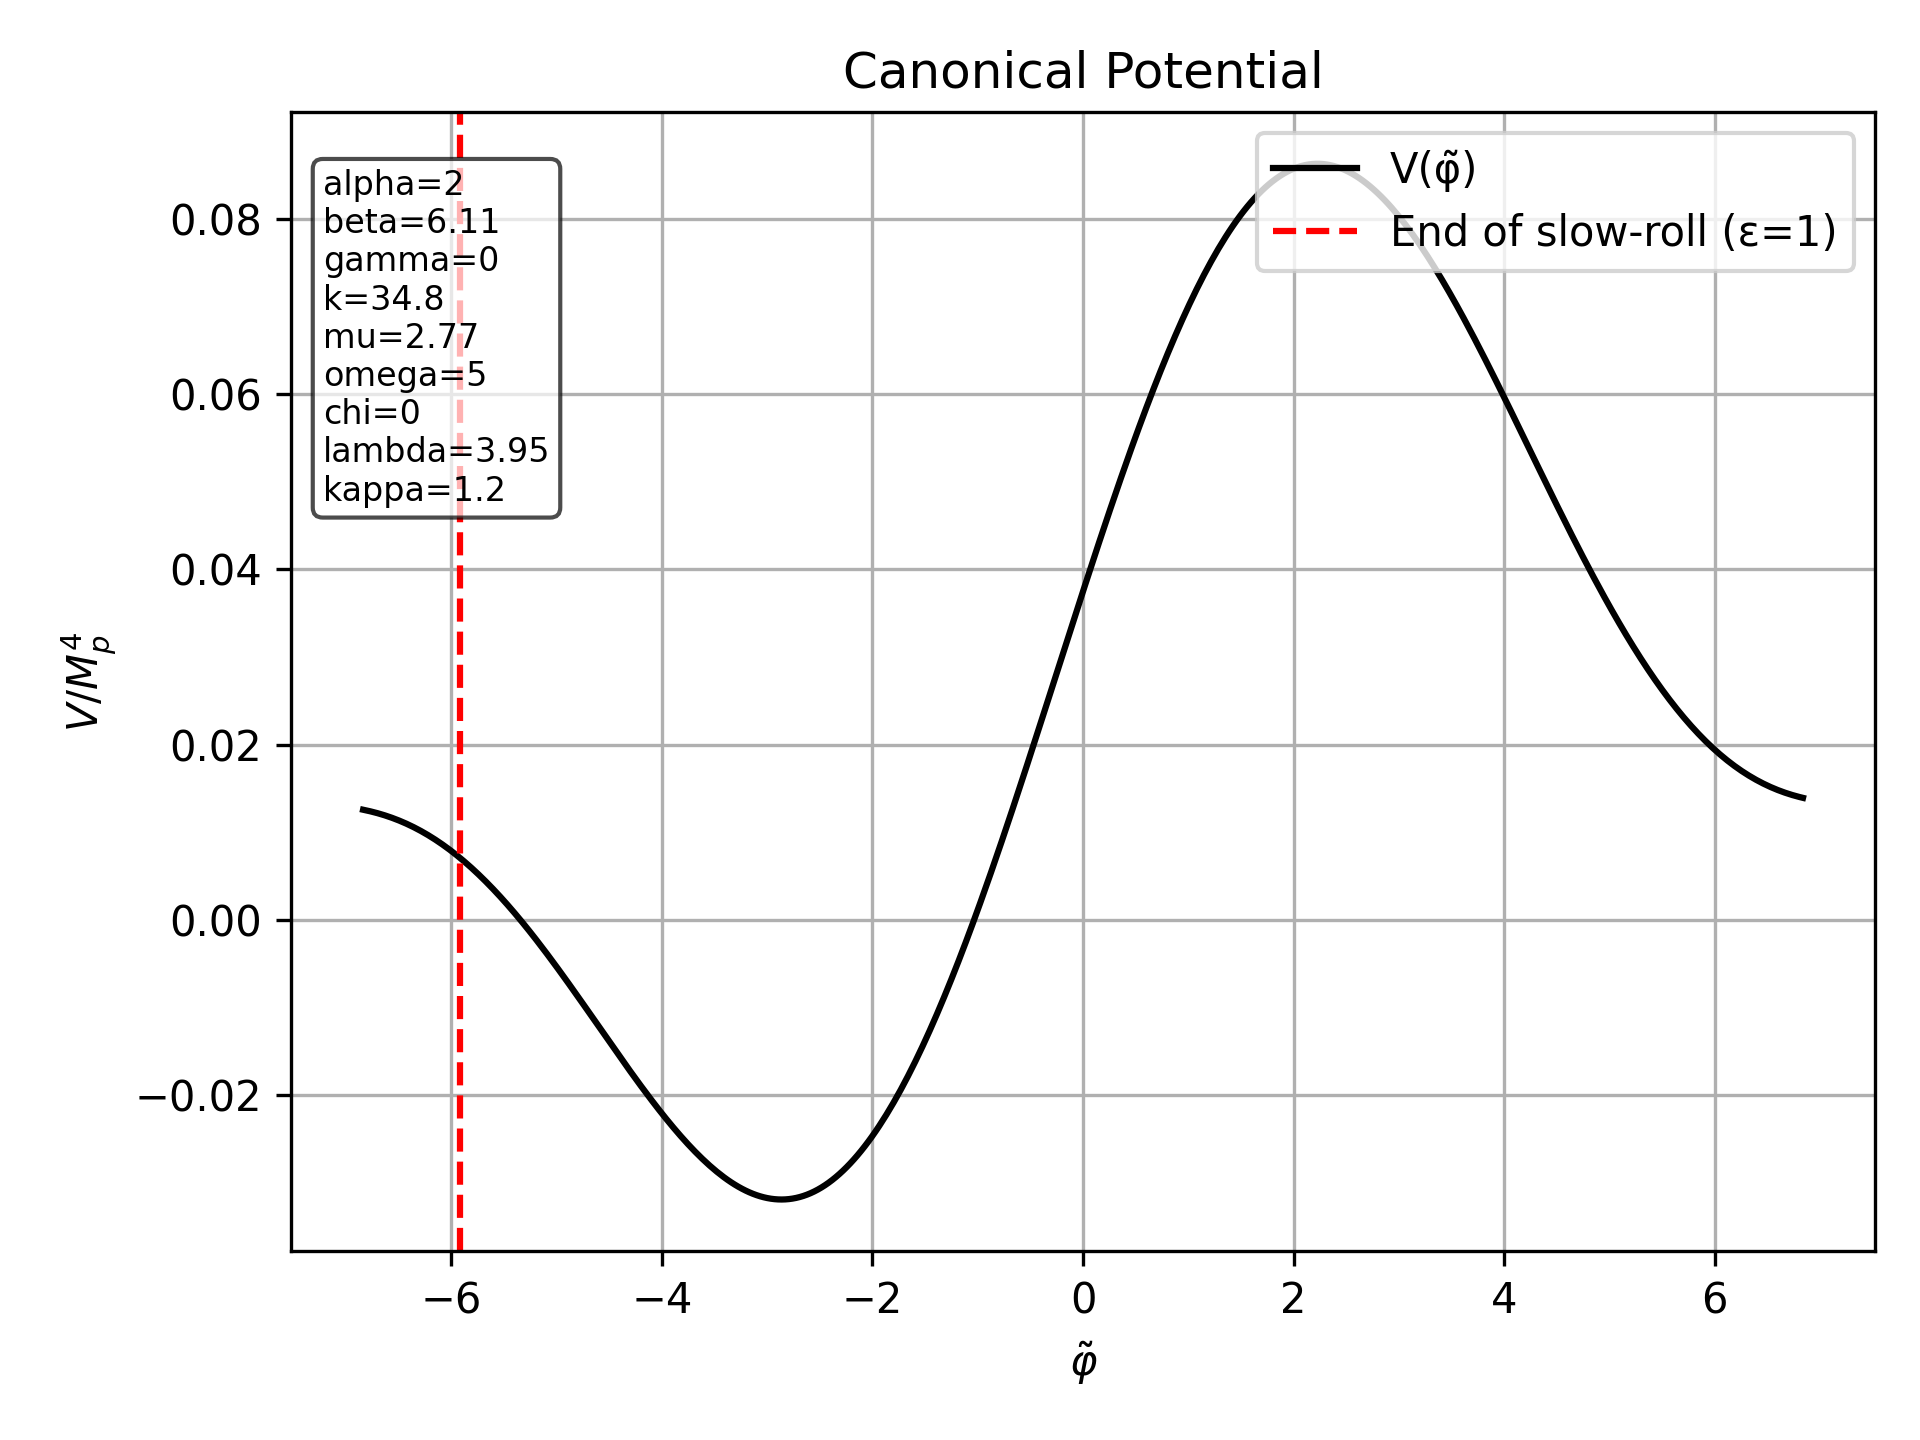
\includegraphics[width=0.4\textwidth]{Python/Figures/AE/inflation_plots/potential.png}
    \caption{$V(\tilde{\varphi})$ vs $\tilde{\varphi}$ (Un-Optimized)}
    \label{Canonical Potential vs Field1}
\end{figure}
\begin{figure}[h!]
    \centering
    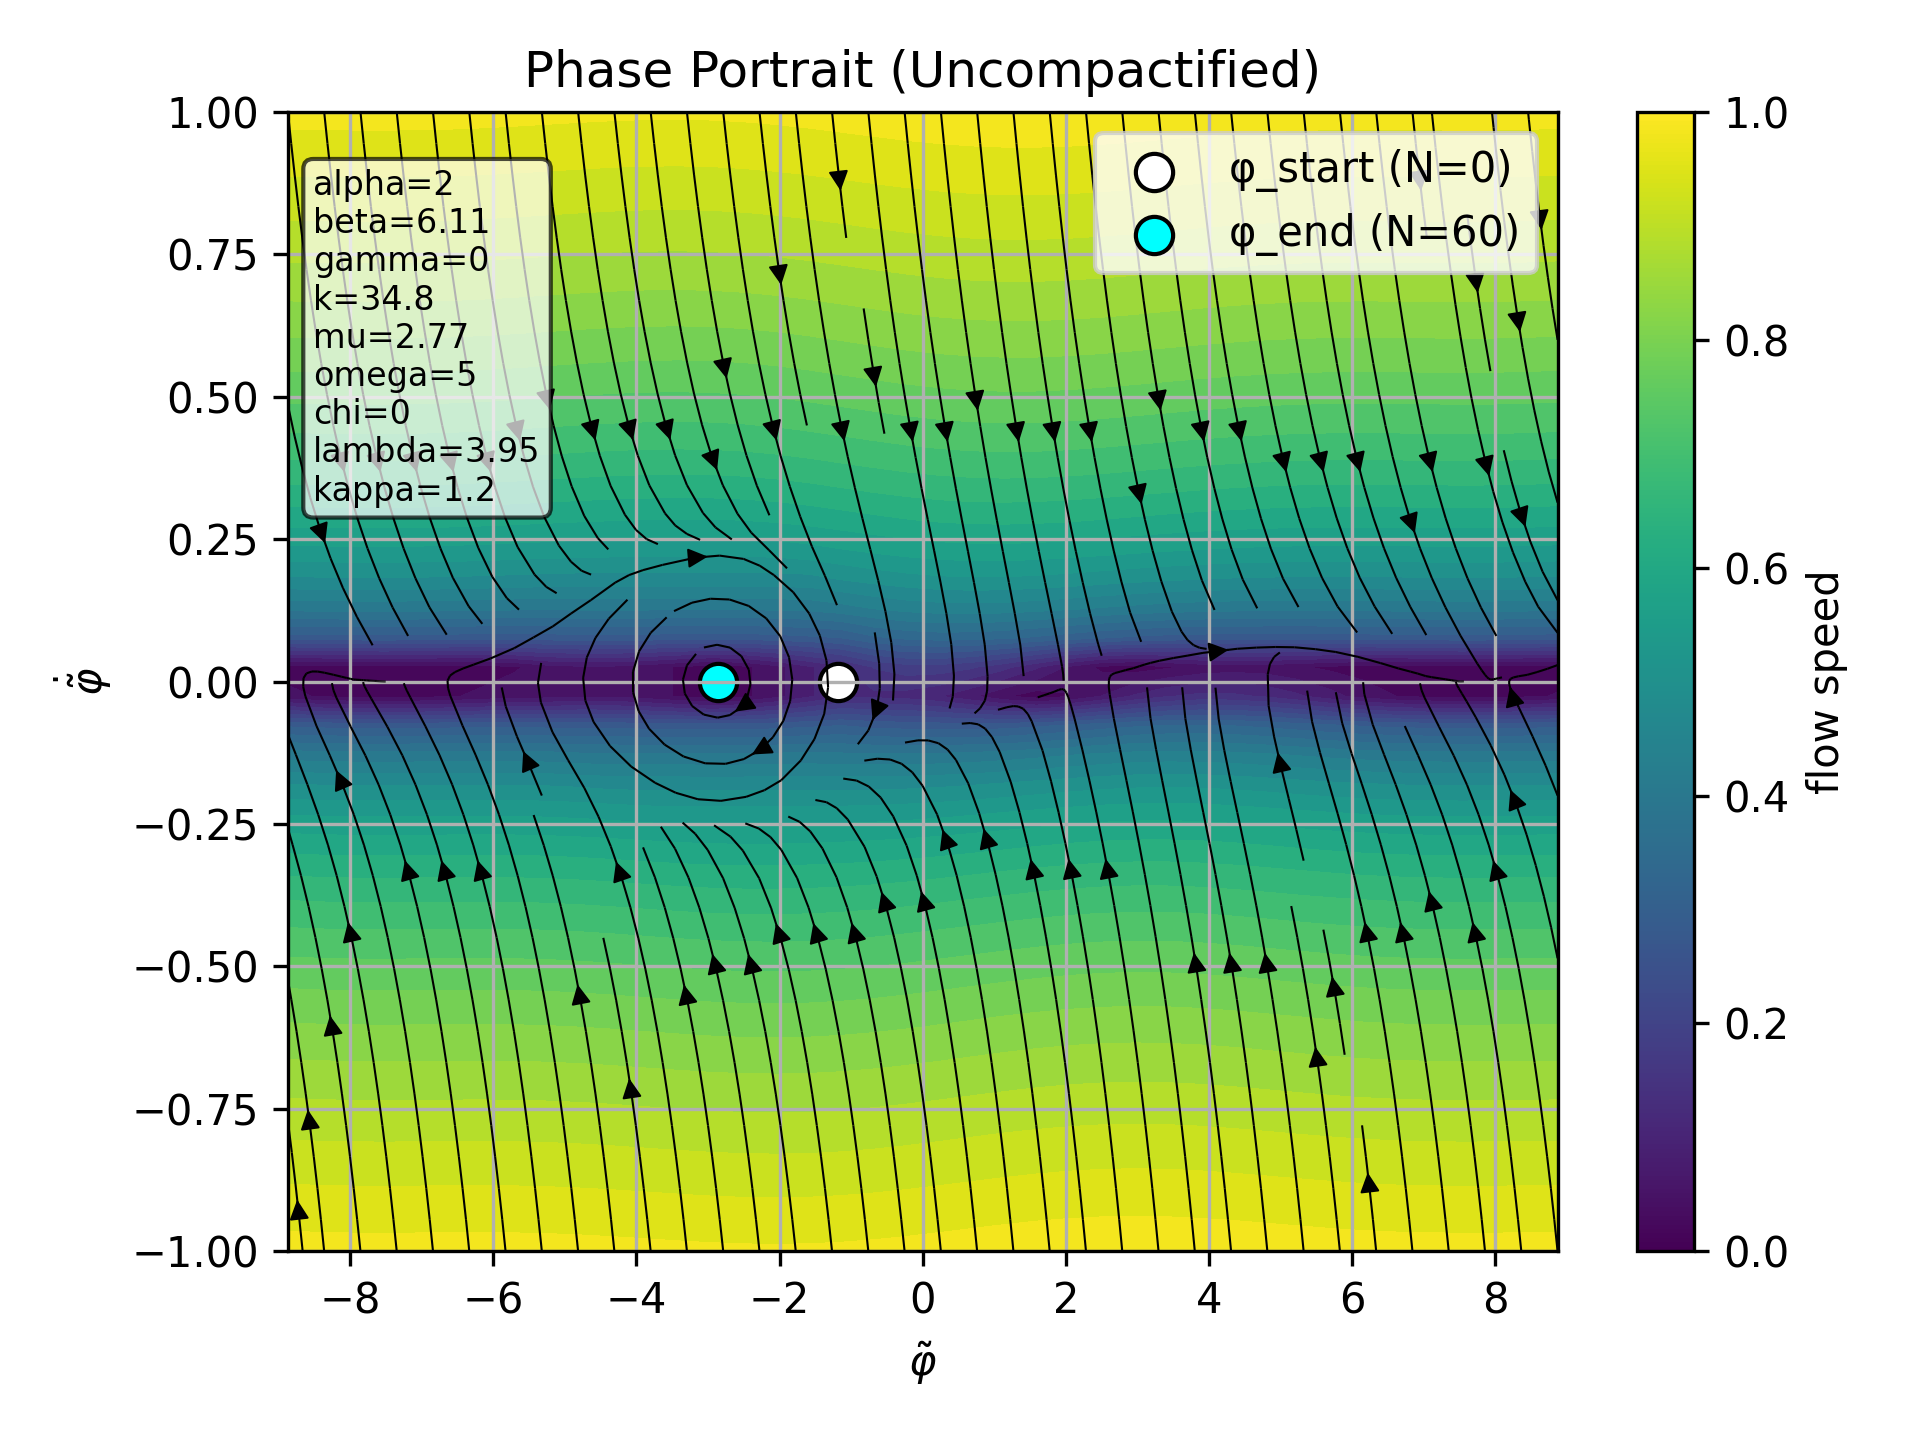
\includegraphics[width=0.5\textwidth]{Python/Figures/AE/inflation_plots/phase_portrait.png}
    \caption{$\dot{\tilde{\varphi}}$ vs $\tilde{\varphi}$}
    \label{Phase Space potrait1}}
\end{figure}

\subsection{Asymptotic Limits} \label{Aymptotic limits}
Analysing this potential, we can see at the limits, $\lim_{X \rightarrow \pm \infty} V(X) \approx \frac{M_p^4}{8} \frac{\lambda}{\beta^2} = V_\infty$. This shows that it plateaus at large $X$ or as $\tilde{\varphi} \rightarrow \frac{\pi}{2 C_k}$, where $C_k = \sqrt{\frac{2}{12+k}} \frac{1}{M_p} = \tilde{\varphi}_\text{max}$.

Building on the ideas of \cite{fairbairn_radion_2003, roest_universality_2014}, which analyse the two universality classes of single-field inflation, we can attempt to get a rough idea of this model's prediction of $n_s \, \text{vs} \, N$ and $r \, \text{vs} \, N$.
Expanding the potential around the plateau (large $X$ or as $\tilde{\varphi} \rightarrow \tilde{\varphi}_{\text{max}}$),
\begin{equation} \label{Asymptotic expansion}
    V(X) \approx \frac{M_p^4}{8} \frac{\lambda}{\beta^2}\left[1 + \frac{B}{X}\right] + \mathcal{O}(X^{-2}),
\end{equation}
where $B = 2(\frac{\chi}{\lambda} - \frac{\gamma}{\beta})$. Denoting $\delta \tilde{\varphi} =  \tilde{\varphi}_{\text{max}} - \tilde{\varphi}$, for small $\delta \tilde{\varphi}$, we get,
\begin{equation}
    \tan(C_k \tilde{\varphi}) \approx \frac{2\beta}{D}X,
\end{equation}
since $\delta \tilde{\varphi} \ll 1$, we get $\tan(C_k \tilde{\varphi}_{\text{max}} - C_k\delta\tilde{\varphi}) = \tan(\frac{\pi}{2} - C_k\delta\tilde{\varphi}) \approx \frac{1}{C_k \delta \tilde{\varphi}}$. Implying therefore, 
$
\frac{1}{C_k \delta \tilde{\varphi}} \approx \frac{2\beta}{D}X
$, using this in \cref{Asymptotic expansion}, we get
\begin{align} \label{Weird Approx}
    V(\tilde{\varphi}) \approx V_{\infty}[1 - B'(\tilde{\varphi}_{\text{max}} - \tilde{\varphi}) + \cdots],
\end{align}
where $V_\infty = \frac{M_p^4}{8} \frac{\lambda}{\beta^2}$ and $B' = \frac{4C_k}{D} (\gamma-\frac{\beta\chi}{\lambda})$. Then re-writing \cref{Weird Approx} as $V(\delta\tilde{\varphi}) \approx V_{\infty} \exp{[\ln(1 - B'(\delta \tilde{\varphi})]} \approx V_\infty e^{-B'\delta \tilde{\varphi}}$. Finally, shifting \(\delta\tilde\varphi\to\tilde\varphi\), giving us the familiar plateau–exponential form:
\begin{equation}
    V(\tilde{\varphi}) \approx V_\infty [1 - e^{-B' \tilde{\varphi}} ] = M^4 (1 - e^{-q\tilde{\varphi}/M_p}).
\end{equation}
In the second equality, we have compared it to the result from models derived in the context of SUSY \cite{stewart_inflation_1995}, string compactification \cite{cicoli_fibre_2009}, brane inflation \cite{dvali_brane_1999}, and summarized in \cite{martin_encyclopaedia_2014}, using similar analysis, we get:
\begin{align}
    n_s &\approx 1 - \frac{2}{N}, \\
    r &\approx \frac{8}{q^2N^2} = \frac{(12+k)(4\alpha\beta - \gamma^2)}{4} \left(\frac{\lambda}{\lambda \gamma - \chi \beta} \right)^2 \frac{1}{N^2}.
\end{align}

\begin{comment}
 we can expand the potential around the plateau, taking the asymptotic value to be the background, that is,

     We can now compare this potential to the well-studied Power-Law inflation models \cite{martin_encyclopaedia_2014} given by:
    \begin{equation}
        V(\tilde{\varphi}) \approx V_\infty e^{-B' \tilde{\varphi}} = M^4 e^{-\alpha' \tilde{\varphi}/M_p}
    \end{equation}
    
    Compared to our model (the $\alpha$ has been primed to distinguish it from the parameter in our model), we get that:
    \begin{align}
        \alpha' &=  \frac{4}{D} \sqrt{\frac{2}{12+k}} \left(\gamma - \frac{\beta\chi}{\lambda} \right) \nonumber \\
        n_s &\approx 1 - \alpha^{'2} \, \, \, \, \,\,\,\,\,\,\, r \approx 8 \alpha^{'2} 
    \end{align}
    Though these models are disfavored as they do not depend on the energy scale at which reheating ends, this analysis provide a rough idea of the behaviour at the edges of the graph, where $X$ is large ($\tilde{\varphi} \approx \frac{\pi}{2 C_k}$), that $n_s$ and $r$ become constant. To understand the behaviour in the entire graph requires more careful and exact analysis.
\end{comment}
\subsection{Simplification of the model} \label{Reduction of parameters}
We observe that these models exhibit behaviour roughly in line with what we would expect from inflationary models. For a more precise analysis, we would need to examine the exact form of the potential \cref{Potential}. This has nine free dimensionless parameters. However, the previous analysis shows us that only certain combinations of parameters affect the observables. To make this exact, we define the new variable $Y$ as:
\begin{align}
    Y(\tilde{\varphi}) &= X(\tilde{\varphi}) + \frac{\gamma}{2\beta}
\end{align}
Denoting $A(X) = \beta X^2 + \gamma X + \alpha$ and $D = \sqrt{4\alpha\beta-\gamma^2}$, we get:
\begin{align}
    A(Y) &= \beta Y^2 + \frac{D^2}{4\beta}
\end{align}
For the numerator $N(X) = \kappa + 2\omega X +\mu X^2 + 2\chi X^3 + \lambda X^4$, following a similar procedure as the denominator above, we get the following redefinition of parameters: 
\begin{subequations}
\begin{align} \label{huge redefiniton}
    \kappa &\rightarrow \kappa - \frac{\gamma\omega}{\beta} + \frac{\gamma^2\mu}{4\beta^2} - \frac{\gamma^3\chi}{4\beta^3} +\frac{\gamma^4\lambda}{16\beta^4}    \\
    2\omega &\rightarrow 2\omega - \frac{\gamma\mu}{\beta} + \frac{3\gamma^2\chi}{2\beta^2} - \frac{\gamma^3\lambda}{2\beta^3}    \\
    \mu &\rightarrow \mu - \frac{3\gamma\chi}{\beta} + \frac{3\gamma^2\lambda}{2\beta^2}  \\
    2\chi &\rightarrow 2\chi - \frac{2\gamma\lambda}{\beta}  \\
    \lambda &\rightarrow \lambda 
\end{align}    
\end{subequations}
Using this redefinition of parameters, we can write the numerator as before, however, with $Y$ as the primary variable, $N(Y) = \kappa + 2\omega Y +\mu Y^2 + 2\chi Y^3 + \lambda Y^4$. Writing down the equations \cref{Potential} and \cref{X}, we see
\begin{align}
    V(Y) &= \frac{M_p^4}{8} \left(\frac{\lambda Y^4 + 2 \chi Y^3 + \mu Y^2  + 2\omega Y + \kappa}{(Y^2 + D^2)^2} \right),  \\
    Y(\tilde{\varphi}) &= D \tan \left(\frac{C \tilde{\varphi}}{M_p} \right),
\end{align}
where, we have performed another implicit redefiniton as $D \rightarrow \frac{D}{2\beta}$, $ \{\lambda, 2\chi, \mu, 2\omega,  \kappa \} \rightarrow \{\lambda, 2\chi, \mu, 2\omega,  \kappa \} /\beta^2$ and denoted $\sqrt{\frac{2}{12+k}} = C$. As a last step, we see that a factor of $D^4$ can be factored from both the numerator and denominator provided we make the identification $\{Y, \lambda, \chi, \mu, \omega, \kappa \} \rightarrow \{Y/D, \lambda, \chi/D, \mu/D^2, \omega/D^3, \kappa/D^4 \}$ to get:
\begin{align}
    V(Y) &=  \frac{M_p^4}{8}  \left(\frac{\lambda Y^4 + 2 \chi Y^3 + \mu Y^2  + 2\omega Y + \kappa}{(Y^2 + 1)^2} \right) ,\label{finalest potential} \\
    Y(\tilde{\varphi}) &=  \tan \left(\frac{C \tilde{\varphi}}{M_p} \right). \label{finalest redef}
\end{align}
Therefore, starting from the equations \cref{Potential} and \cref{X} with nine parameters, we were able to reduce our model to one with only 6, as shown in \cref{finalest potential} and \cref{finalest redef}. $\{\alpha, \gamma,\beta, k , \mu, \omega, \chi, \lambda, \kappa\} \rightarrow \{C , \mu, \omega, \chi, \lambda, \kappa\}$. The original conditions on the parameters and variables get inherited by this new set as $\tilde{\varphi} \in (-\frac{\pi M_p}{2C},\frac{\pi M_p}{2C})$, $Y \in (-\infty,\infty)$ and $C > 0$. We can simplify the potential \cref{finalest potential} and write it directly as a function of $\tilde{\varphi}$ as:

\begin{widetext}
    \begin{equation} 
    \begin{aligned} \label{Ugliest full Potential}
        V(\tilde{\varphi}) =  \frac{M_p^4}{8} \Bigg(\lambda \sin^4\left( \frac{C \tilde{\varphi}}{M_p}\right) + 2 \chi \sin^3\left( \frac{C \tilde{\varphi}}{M_p}\right) \cos\left( \frac{C \tilde{\varphi}}{M_p}\right)  + \mu \sin^2\left( \frac{C \tilde{\varphi}}{M_p}\right) \cos^2\left( \frac{C \tilde{\varphi}}{M_p}\right) + 2\omega \sin\left( \frac{C \tilde{\varphi}}{M_p}\right) \cos^3\left( \frac{C \tilde{\varphi}}{M_p}\right)  \\ + \kappa \cos^4\left( \frac{C \tilde{\varphi}}{M_p}\right) \Bigg)
    \end{aligned}
\end{equation}
\end{widetext}
The only assumption in this process was that $\beta \neq 0$, which is required for $D > 0$. The mapping of these new dimensionless parameters at the end in \cref{Ugliest full Potential} to the original ones we started with in \cref{Potential} has been given in the \cref{Mapping of Parameters}. Denoting $\frac{C\tilde{\varphi}}{M_p}$ as $\theta$, the first and second derivatives of this potential are given by:
\begin{comment}
\wb{What does this mean?}

    We also see that for small values of $C$, we get an approximate shift symmetry in our potential \cite{finelli_effective_2018}\wb{What does this mean?}.
\end{comment}
\begin{widetext}
    \begin{subequations} 
        \begin{align} \label{Derivatives of Pot}
            \frac{\text{d}V}{\text{d}\tilde{\varphi}} &= \frac{CM_P^3}{8} \left[ (-\chi + \omega) \cos4\theta + (-\kappa + \lambda) \sin2\theta + \cos2\theta (\chi + \omega - (\kappa + \lambda - \mu ) 
            \sin2\theta) \right] , \\
            \frac{\text{d}^2V}{\text{d}\tilde{\varphi}^2} &= -\frac{C^2M_P^2}{4} \left[ (\kappa - \lambda) \cos2\theta + (\kappa + \lambda - \mu) \cos4\theta + (\chi+\omega) \sin2\theta + 2(-\chi + \omega) \sin4\theta \right]. 
        \end{align}
    \end{subequations}
\end{widetext}
To analyse the the effective mass of the inflaton, we shall make the simplifying assumption that the minimum of the potential occurs at zero (i.e., $V_{,\tilde{\varphi}} = 0$, this is not a general analysis and is a particular regime of solutions we are choosing to focus on) for that, we require $\omega = 0$.
Using this in the formula for the second derivative, we get:
\begin{equation}
    m_{\tilde{\varphi}}^2 \approx  \frac{\text{d}^2V}{\text{d}\tilde{\varphi}^2} \Bigg|_0 = \frac{C^2M_p^2}{4}(  \mu - 2\kappa)
\end{equation}
This result is exact for the given potential if we set $\omega = 0$. Again, by mass, we refer to the coefficient of the quadratic term in the potential (See \cref{Footnote 1}). We require $m_{\tilde{\varphi}}^2 > 0$ to allow for reheating, as this corresponds to $V_{,\tilde{\varphi}\tilde{\varphi}} > 0$; a minimum around which the inflaton field can oscillate.

\begin{comment}
    This last redefiniton and form of the potential \cref{final potential} and \cref{final redefiniton} essentially help us reduce our parameter list further by two $\{\alpha, \gamma,\beta, k , \mu, \omega, \chi, \lambda, \kappa\} \rightarrow \{D, C , \mu, \omega, \chi, \lambda, \kappa\}$. The original conditions on the parameters and variables get inherited by this new set as $Y \in (-\infty,\infty)$ and $D, C > 0$
    
    We have therefore reduced our parameter list by one $[\alpha, \gamma,\beta, k , \mu, \omega, \chi, \lambda, \kappa] \rightarrow [D, \beta , k , \mu, \omega, \chi, \lambda, \kappa]$

    
    Denoting $A(X) = \beta X^2 + \gamma X + \alpha$, $N(X) = \kappa + 2\omega X +\mu X^2 + 2\chi X^3 + \lambda X^4$ and $D = \sqrt{4\alpha\beta-\gamma^2}$, we get that the slow roll parameter $\epsilon_V$ is:
    \begin{align}
        \epsilon_V(\tilde{\varphi}) &= \frac{2 M_p^2}{C_k^2 D^2} \left[ \frac{N'(X)}{N(X)} - \frac{A'(X)}{A(X)} \right]^2 
    \end{align} 
\end{comment}



\begin{comment}
    \epsilon_V &= \frac{4M_p^4}{(12+k)(4\alpha\beta-\gamma^2)} \left[ \frac{2\omega + 2\mu X + 6\chi X^2 + 4\lambda X^3}{\kappa + 2\omega X +\mu X^2 + 2\chi X^3 + \lambda X^4 } - \frac{2 \beta X + \gamma}{\beta X^2 + \gamma X + \alpha} \right]^2
    


    $\text{params} = [\alpha, \gamma,\beta, \epsilon, \sigma, \nu , \mu, \omega, \chi, \lambda, \kappa]$
    After the variable parameterization, now only 4 dimensionless parameters remain free; $\{\alpha, \gamma,\beta, \epsilon, \sigma , \nu\} \rightarrow \{k, \beta, \gamma, \alpha \}$.
    So now $\text{params} = [\alpha, \gamma,\beta, k , \mu, \omega, \chi, \lambda, \kappa]$
    \begin{equation}
        \begin{Bmatrix}
            \epsilon \\ \sigma \\ \nu 
        \end{Bmatrix}
        = (12+k)
        \begin{Bmatrix}
            \beta \\ \gamma \\ \alpha
        \end{Bmatrix}
    \end{equation}
    \begin{align}
        V({\tilde{\varphi}}) &= M^4  \frac{ \kappa \phi_0^4 + 2\omega \phi_0^3 \tilde{\varphi} +\mu^2 \phi^2_0 \tilde{\varphi}^2 + 2\chi \phi_0 \tilde{\varphi}^3 + \lambda \tilde{\varphi}^4 }{2(\beta \tilde{\varphi}^2 + \gamma\phi_0\tilde{\varphi} + \alpha \phi_0^2)^2} \nonumber \\
        \varphi(\tilde{\varphi}) &= \frac{\phi_0}{2\beta} \Biggl[ \sqrt{4\alpha\beta - \gamma^2} \tan\left(\sqrt{\frac{2}{12+k}}\frac{\tilde{\varphi}}{M_p}\right) - \gamma \Biggr] 
    \end{align}    
    \wb{You should point to these again using cref} 
\end{comment}

\paragraph*{Numerical Analysis}
Optimizing the parameters such that at $N=60$, we get $n_s = 0.9649$, we get the below graphs \cref{Optimized Canonical Potential vs Field1}, \cref{Optimized Phase Space potrait1} and \cref{Optimized Compact Phase Space potrait1} (We have set $M_p = 1$ for these graphs and code):
\begin{figure}[h!]
    \centering
    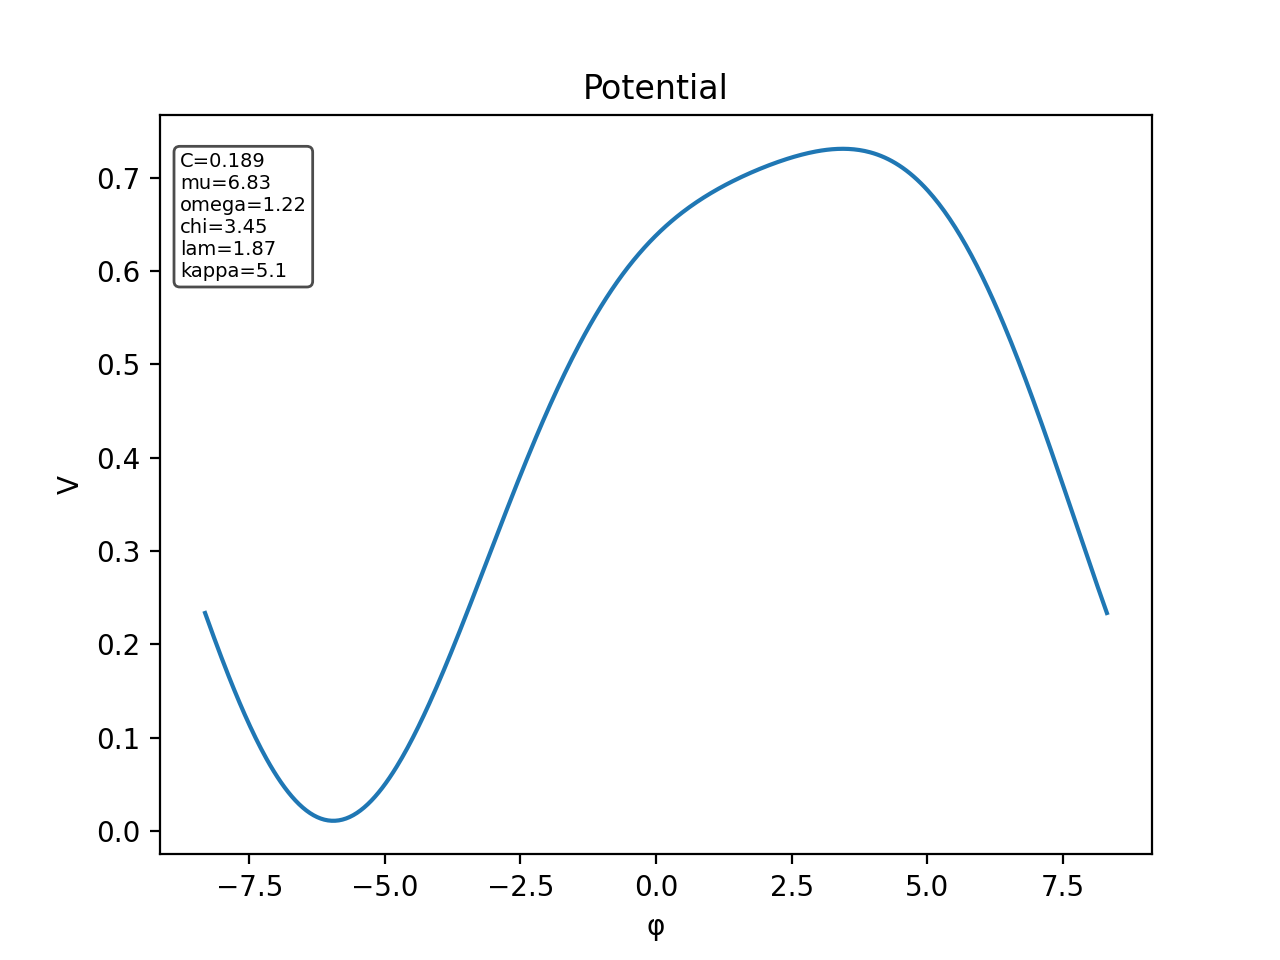
\includegraphics[width=0.5\textwidth]{Python/results/potential.png}
    \caption{$V(\tilde{\varphi})$ vs $\tilde{\varphi}$ (Optimal Coefficients)}
    \label{Optimized Canonical Potential vs Field1}
\end{figure}
\begin{figure}[h!]
    \centering
    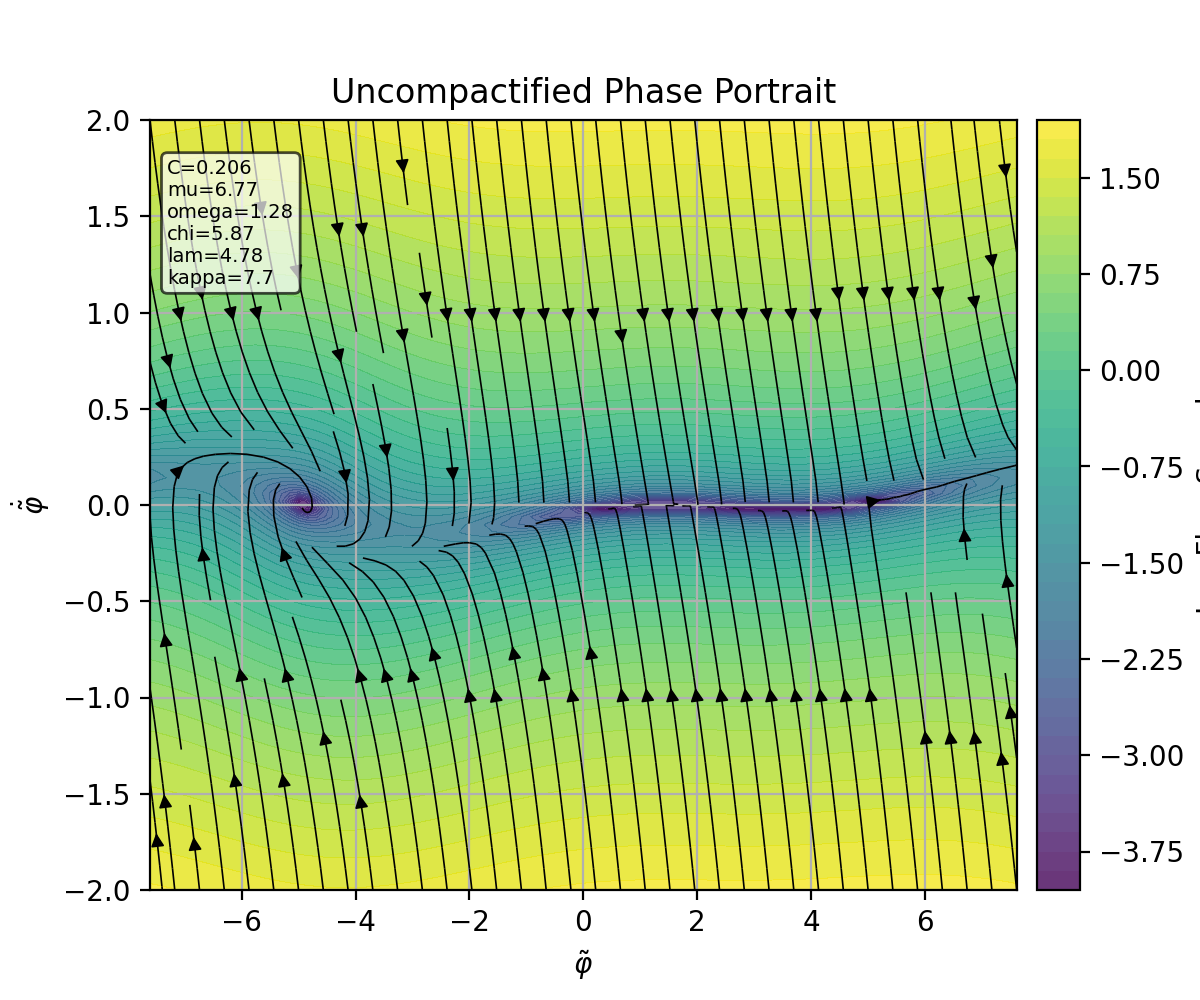
\includegraphics[width=0.5\textwidth]{Python/results/phase_uncompact.png}
    \caption{$\dot{\tilde{\varphi}}$ vs $\tilde{\varphi}$}
    \label{Optimized Phase Space potrait1}}
\end{figure}
\begin{figure}[h!]
    \centering
    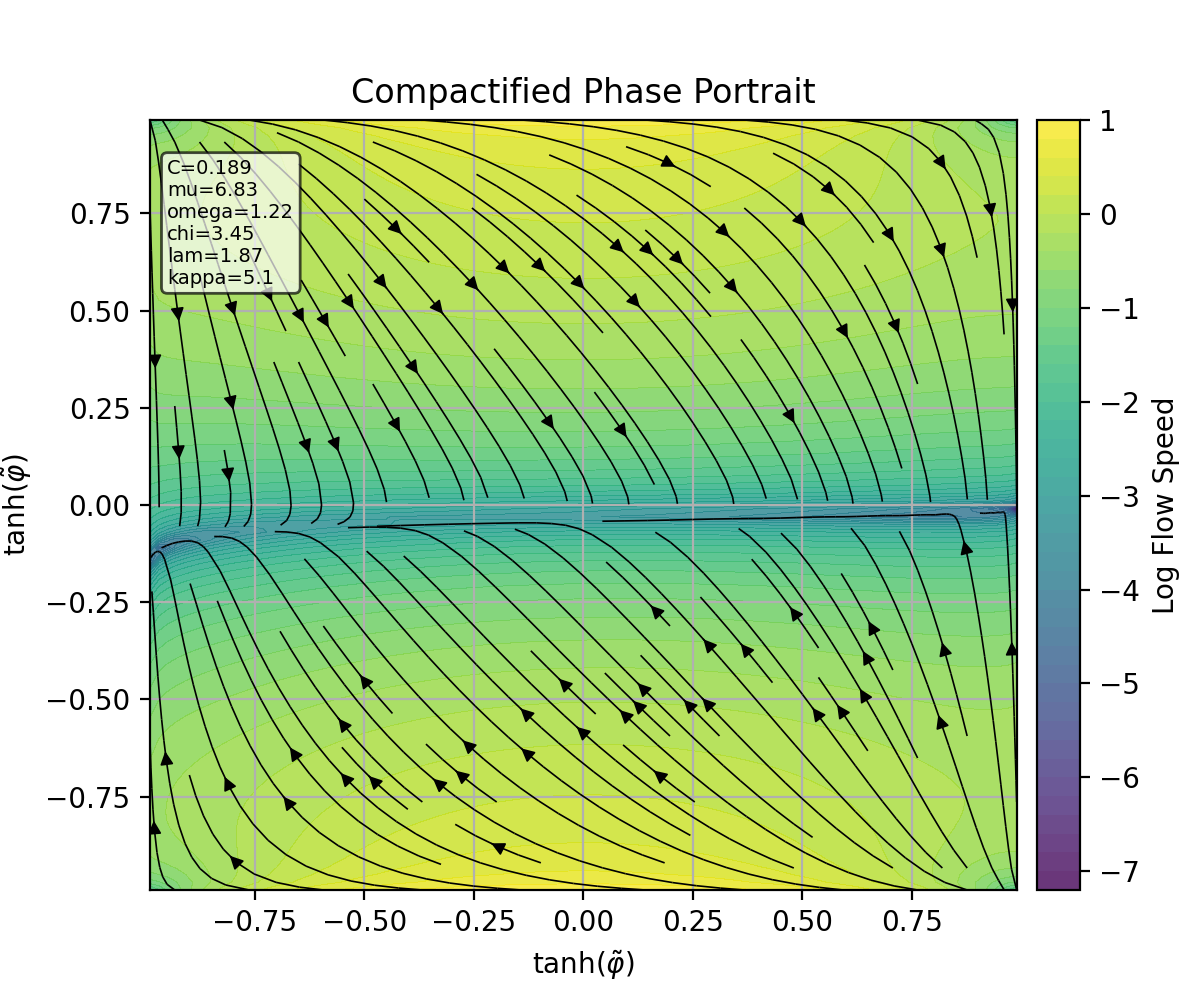
\includegraphics[width=0.5\textwidth]{Python/results/phase_compact.png}
    \caption{$\dot{\tilde{\varphi}}$ vs $\tilde{\varphi}$ (Compactified)}
    \label{Optimized Compact Phase Space potrait1}}
\end{figure}

The phase space portrait (\cref{Optimized Phase Space potrait1}) clearly shows attractor behaviour at the minima of the potential (\cref{Optimized Canonical Potential vs Field1}) at $\tilde{\varphi}_0 \approx -4.9157 M_p$. For these parameters, the mass of the inflaton is $m_{\tilde{\varphi}}^2 \approx  0.1965 M_p^2$. For the value of $C = 0.2063$, we get that the range of the canonical field is $\tilde{\varphi} \in (-7.61414,7.61414)$. The only caveat with the portrait is that it shows trajectories exiting and entering this range. We would expect something akin to the trajectories in the compactified phase space \cref{Optimized Compact Phase Space potrait1}. However, this is not a failure of the theory. While plotting, we have used the EOMs \cref{KGEOM} and \cref{Friedmann 3}, which means treating $\tilde{\varphi}$ as the fundamental field without any bounds.


\section{CONCLUSION}
We have shown that by demanding local scale invariance in a gravity-scalar theory and analysing the most general action that is linear in curvature, we get a potential that lends itself to be uniquely interpreted as an inflaton potential. We did this by introducing a gauge boson to account for the new Weyl gauge symmetry. We also had to introduce one compensator field to give rise to the quadratic minima we wanted our potential to have. This sets the energy scale at which scale invariance is broken.

An important consequence of our results is that the energy scale at which scale invariance is broken drops out and does not affect our observables. This avoids the common pitfalls of adding an arbitrary energy scale to our theory by hand and avoids the criticism levied against such models as described in \cref{Footnote Criticism}. It also shows that the gauging of scale invariance in our theory leads to universal behaviour regardless of the energy scale.

We have also demonstrated that, at least classically, such models contain redundant parameter choices that yield the same physics. 

The Python optimizer code, plotter code, and the Mathematica notebooks, which have been used to verify these calculations, have been uploaded to the GitHub Repository, which is available as supplemental material. 
\begin{comment}
    \wb{Not sure what regularly means here.} \pcs{removed} 
\end{comment}
\newpage
\,\,
\newpage

%TC:ignore
\appendix
\section{A Primer on Inflaton}\label{The need for Inflation}

\subsection{Horizon Problem} \label{Horizon Problem}
In this section, we will show that given the standard assumed expansion rate in the Big Bang model, we cannot satisfactorily explain the near-perfect uniformity of the CMB. This is because, given the rate of expansion, there is no way for distant regions of the CMB to have once been causally connected.
Given the Friedmann Equations and defining the Hubble constant $H = \frac{\dot{a}}{a}$,
\begin{align}    
    \ddot{a} &= -\frac{4\pi G}{3} (\rho + 3p)a \label{Friedmann Eqn 1} \\
    H^2 + \frac{k}{a^2} &= \frac{8 \pi G}{3} \rho \label{Friedmann Eqn 2} \\
    \dot{\rho} &= -3(\rho + p)H \label{Friedmann Eqn 3}
\end{align}
From the continuity equation \cref{Friedmann Eqn 3}, we have:
\begin{equation} \label{4}
    \frac{\mathrm{d}  \ln(\rho)}{\mathrm{d} \ln(a)} = -3(1+w)
\end{equation}
Where, $w = \frac{p}{\rho}$. We can solve this equation to get $\rho \propto a^{-3(1+w)}$. In combination with the Friedmann equation \cref{Friedmann Eqn 2} for a flat universe $k = 0$, we get the scale factor $a$ as a function of time $a(t)$.
\begin{equation}    \label{5}
    a(t) = \begin{cases}
        t^{2/3(1+w)} & w \neq -1 \\
        e^{Ht} & w = -1
    \end{cases}
\end{equation}
Now, we can define the comoving horizon ($\tau$) as the causal horizon or the maximum distance a light ray can travel between times 0 and $t$.
\begin{equation}    \label{6}
    \tau \equiv \int_{0}^{t} \frac{\mathrm{d} t'}{a(t')} = \int_{0}^{a} \frac{\mathrm{d}a}{H a^2} = \int_{0}^{a} \mathrm{d} \ln(a) \frac{1}{aH}
\end{equation}
Therefore, for a conventional Big Bang model, the causal horizon $\tau$ for a universe with $w \geq 0$ increases with time. This means that the fraction of the universe in contact with each other increases with time.
\begin{equation}
    \tau \propto a^{1/2(1+3w)} \implies \tau = \begin{cases}
        a & \text{Radiation Dominated} \\
        a^{1/2} & \text{Matter Dominated}
    \end{cases}
\end{equation}
The comoving horizon increasing with time implies that comoving scales (comoving scale is not the same as the physical scale) entering the cosmic horizon now were not in causal contact during the CMB decoupling! However, the anisotropy of the CMB is about one part in $10^{-5}$, posing a problem to the conventional big bang model to explain how these distant regions of the CMB managed to regulate their temperatures to such an accurate degree.

\subsection{Flatness Problem} \label{Flatness Problem}
Despite the presence of mass and energy in our universe, the large-scale structure of our spacetime is approximately Euclidean (flat). To see whether this is a stable equilibrium, we return to Friedmann equation \cref{Friedmann Eqn 2} and defining $\rho_{\text{crit}} = 3H^2(a)$ and $\Omega(a) = \frac{\rho(a)}{\rho_{\text{crit}}}$, we get
\begin{equation}
    1 - \Omega(a) = \frac{-k}{(aH)^2}
\end{equation}
Differentiating this equation and using the Friedmann equations, we get,
\begin{equation}
    \frac{\mathrm{d}\Omega}{\mathrm{d} \ln a} = (1+3w)\Omega(\Omega-1)
\end{equation}
Looking at this, we can see that $\Omega = 1  \implies \rho = \rho_{crit}$ is an unstable equilibrium and slight perturbations can make the universe not flat, i.e., $k \neq 0$. This means that in the standard big bang model, matter density has to be extremely fine-tuned to fit the requirement $\rho = \rho_{crit}$, which seems unlikely.

The theory of inflation attempts to resolve the need for extreme fine-tuning of the initial conditions of the universe by positing a period of exponential expansion. The next section shows how this theory solves the two problems stated above.

\subsection{Inflationary Observables}  \label{Inflationary Observables}
Inflation is a robust theory not only because it solves the horizon and flatness problems (See \cref{Horizon Problem}, \cref{Flatness Problem} for more details), but it also makes predictions about the inhomogeneities in the early universe. These primordial density fluctuations are a result of the inherent quantum nature of the inflaton field. 
The fluctuations in the inflaton field $\delta\varphi$ cause different patches of spacetime to have different amounts of inflation as the field has not exited slow-roll in certain regions yet. 

These fluctuations can be treated as perturbations around a background field ($\delta\varphi(t,\textbf{x}) = \varphi(t,\textbf{x}) - \Bar{\varphi}(t)$). However, as is known, by the EFEs $\delta G_{\mu\nu} = \frac{1}{M_p^2}\delta T_{\mu \nu}$, perturbations in the matter density cause perturbations in the metric too. Therefore, we can expand the metric around it's background value similarly as $g_{\mu\nu}(t,\textbf{x}) = \Bar{g}_{\mu\nu}(t) + \delta g_{\mu\nu}(t,\textbf{x})$. Generally, these metric perturbations $\delta g_{\mu\nu}(t,\textbf{x})$ have 10 independent components, but these can be decomposed into scalar, vector, and tensor (SVT) perturbations \cite{liddle_cosmological_2000, malik_cosmological_2009}. Using conformal time and writing the background metric in the same form as \cref{deSitter Conformal}, we get the perturbation to the metric to be of the form
\begin{equation} \label{Perturbed metric}
    \delta g_{\mu\nu}
    = 
    -a^2
    \begin{pmatrix}
        -2 \Phi & \partial_iB \\
        \partial_iB & (1-2\Psi)\delta_{ij} + E_{ij} 
    \end{pmatrix}
\end{equation}
Where $E_{ij} = 2\partial_i\partial_j E + h_{ij}$. There are 4 independent contributions $(\Phi, B, \Psi, E)$ which behave as scalars under transformation of frames and the transverse, traceless ($h_i^i = \partial^ih_{ij} = 0$), and symmetric tensor contribution $h_{ij}$ to the perturbed metric. We have neglected terms corresponding to the vector perturbations as they are not created by inflation, and as they also decay with the expansion of the universe. The reason we would prefer to split the metric perturbation into these three types is that at linear order, the Fourier modes decouple, and we can analyse them separately. 


However, with a change in coordinates, while the tensor contributions remain the same, the scalar functions change. Therefore, by a suitable choice of coordinates, we could remove the inhomogeneities in the inflaton field $\delta \varphi(\textbf{x}',t') = 0$. To analyse these perturbations, it is therefore important to consider gauge-invariant quantities. An obvious choice would be to consider the intrinsic curvature of the spatial hypersurface ${}^{(3)}R$ (See \cref{3+1 decomposition of spacetime}). However, it is easier to work with a related quantity that makes no reference to the scale factor and is normalised. This quantity can therefore be defined as
\begin{equation} \label{comoving curvature perurbation}
    \mathcal{R} \equiv 4 \frac{k^2}{a^2} {}^{(3)}R = \Psi - \frac{H}{\dot{\Bar{\varphi}}}\delta \varphi
\end{equation}
This is called the comoving curvature perturbation ($k$ here corresponds to the wavenumber of the Fourier mode). Another quantity of interest is the two polarization modes of the tensor perturbation $h_{ij}$, that is, $h \equiv h^+ , h^\times$, these are the gravitational waves generated due to inflation. The observables we can constrain from these two quantities are the scalar and tensor power spectra ($P_\mathcal{R}(k)$ and $P_h(k)$), respectively
\begin{align}
    \langle \mathcal{R}_{\bm{k}} \mathcal{R}_{\bm{k}'} \rangle &= (2\pi)^3 \delta(\bm{k}+\bm{k}')P_\mathcal{R}(k) \\
    \langle h_{\bm{k}} h_{\bm{k}'} \rangle &= (2\pi)^3 \delta(\bm{k}+\bm{k}')P_h(k)
\end{align}
Where $\bm{k}$ is the Fourier wavevector corresponding to that mode in the decomposition. Defining $\Delta_s^2 = \frac{k^3}{2\pi^2} P_\mathcal{R}(k)$ and $\Delta_t^2 = \frac{k^3}{\pi^2} P_h(k)$ (upon summing over the two polarizations, we lose a factor of 2 in the denominator in the definition of $\Delta_t^2$), we get the scale-dependence of the power spectrum, often called the scalar tilt as follows
\begin{equation}
    n_s - 1 \equiv \frac{\text{d} \ln \Delta_s^2}{\text{d} \ln k}
\end{equation}
and the tensor-to-scalar ratio, which is defined as the normalized value of the amplitude of the tensor fluctuations with respect to the amplitude of the scalar fluctuations
\begin{equation}
    r \equiv \frac{\Delta_t^2(k)}{\Delta_s^2(k)}
\end{equation}
The scalar tilt (also called the scalar spectral index) measures how the curvature perturbation spectrum scales with wavenumber $P_\mathcal{R}(k) = A_s\big(\frac{k}{k_*}\big)^{n_s-1}$, where $A_s$ is the amplitude of the scalar perturbation and $k_*$ is the pivot scale, the comoving wavenumber at which the the amplitude is defined. $n_s = 1$ corresponds to a scale-invariant spectrum (Harrison‑Zeldovich \cite{harrison_fluctuations_1970, zeldovich_hypothesis_1972, peebles_primeval_1970})
. $n_s < 1$ implies that there is more power at smaller $k$ (larger scales) and $n_s > 1$ implies that there is more power at larger $k$ (smaller scales). 
\
The latest Planck data \cite{collaboration_planck_2020} constrains these values to around $n_s = 0.9649 \pm 0.0042$, which strongly rules out the Harrison‑Zeldovich spectrum with a confidence of $8.4\sigma$. However, it still shows that the spectrum is \textit{nearly} scale-invariant, with $P_\mathcal{R}(k) \propto k^{-0.0351}$. For $r$, the Planck data constrains the upper limit to $r_{0.002} < 0.056$ at the pivot scale $k_* =0.002 \text{Mpc}^{-1}$
\begin{comment}
    \wb{So in general, you want to put some punctuation at the end of each equation, and avoid punctuation at the end of the line before the equation. Exceptions apply for very large displayed equations.}

    \wb{Typo.}
\end{comment}
At leading order, the power spectrum is related to the slow-roll parameters by \cite{liddle_cosmological_2000}
\begin{equation}
    P_\mathcal{R}(k) \approx \frac{1}{24\pi^2 M_p^4} \frac{V}{\epsilon_V}
\end{equation}
Using the slow roll condition $\text{d}t = -(3H/V') \text{d}\varphi$, we find
\begin{equation}
    \frac{\text{d}}{\text{d} \ln k} \epsilon_V = -M_p^2 \frac{V'}{V}\frac{\text{d}}{\text{d}\varphi}\epsilon_V = 2\epsilon_V\eta_V - 4\epsilon_V^2
\end{equation}
Putting this together, we get $n_s \approx 1 -6\epsilon_V +2\eta_V$, and similar analysis \cite{baumann2012tasilecturesinflation} gives us $r \approx 16 \epsilon_V$ at the horizon crossing scale $k = aH$.


\section{Translating variables from the papers \cite{Salvio_2022} to \cite{barker2024poincaregaugetheoryconformal}} \label{Appendix A}
In the paper \cite{Salvio_2022}, the authors derived an inflaton potential using metric-affine gravity. The motivation here is to give inflation a geometrical explanation. 
By starting with this action, 
\begin{equation}
    S = \int \text{d}^4\text{x} \sqrt{-g} (\alpha \mathcal{R} + \beta \mathcal{R}' + c' \mathcal{R}'^{2})
\end{equation}
Where $\mathcal{R}'$ is the Holst Invariant, a \textit{scale-invariant} quantity. The potential derived finally is: 
\begin{equation}
    U_S(\omega) = \frac{1}{4 c'} \left[ \frac{M_{p}^{2}}{4} \text{sinh}(\text{X}_S(\omega)) - \beta  \right]^2
\end{equation}
where
\begin{equation}
    \text{X}_S(\omega) = \sqrt{\frac{2}{3}} \frac{\omega}{M_{p}} + \text{tanh}^{-1} \left(\frac{4 \beta}{\sqrt{M_{p}^{4}+16 \beta^2}} \right)
\end{equation}
In \cite{barker2024poincaregaugetheoryconformal}, the authors derive a similar form of the potential starting with a scale-invariant scalar field action. The resulting potential is:
\begin{equation}
    U_B(\varphi) = \frac{\mu^2 \phi_{0}^{4}}{2} \left[ \frac{\sigma}{2} + \sqrt{\nu - \frac{\sigma^2}{4}} \text{sinh}\left( \text{X}_B(\varphi) \right)  \right]^2
\end{equation}
where
\begin{equation}
    \text{X}_B(\varphi) =  \frac{\varphi}{\phi_0 \sqrt{\nu - \frac{\sigma^2}{4}}} - \frac{c}{\phi_0 \sqrt{\nu - \frac{\sigma^2}{4}}}
\end{equation}
The substitutions necessary to transform back and forth from these models are: 
\begin{subequations}
    \begin{align}
    \phi_0 &= g \sqrt{\frac{3}{2}} M_p , \\
    \mu &= g^{-1} \frac{1}{6 \sqrt{2 c'}}, \\
    \sigma &= - g^{-1} \frac{8 \beta}{M_{p}^{2}} , \\
    \nu &= g^{-2} \left( 1 + \frac{16 \beta^2}{M_{p}^{4}} \right) , \\
    c  &= -\sqrt{\frac{3}{2}} M_{p} \text{tanh}^{-1} \left(\frac{4 \beta}{\sqrt{M_{p}^{4}+16 \beta^2}} \right).
\end{align}
\end{subequations}

Where $g$ is a dimensionless parameter, this tells us that the model in \cite{barker2024poincaregaugetheoryconformal} has an extra redundant parameter that we can absorb into the definitions of the other variables.

\section{Non-Canonical Scalar Field Inflation} \label{Non-Canonical Scalar Field Inflation}

A good part of this project was spent analysing a non-canonical scalar field. To do so, machinery distinct from the one displayed in \cref{Inflation} was required. The following is the derivation for the same. Some of the equations derived have not been found elsewhere in literature (like the EOM for $\varphi$ as a function of N \cref{Kphi vs N})
\begin{equation} \label{13}
    S = \int \text{dt}\text{d}^3\text{x} \; \text{a}^3(t) \left[ \frac{K(\varphi)}{2}\dot{\varphi}^2 - V(\varphi) \right]
\end{equation}
We vary the action, and upon integrating by parts, we get,
\begin{equation}
    \delta S = - \int \text{dt}\,\text{d}^3\textbf{x} \; \left[ a^3 K \ddot{\varphi} + a^3K_{,\varphi} \frac{\dot{\varphi}^2}{2}  +  3\dot{a} a^2 K \dot{\varphi} + a^3V_{,\varphi}  \right]\delta \varphi
\end{equation}
Setting this variation to zero, we get the equation of motion for a non-canonical scalar field.
\begin{equation} \label{16}
    K \ddot{\varphi} + \dot{\varphi} \left(\frac{K_{,\varphi} \dot{\varphi}}{2} + 3H K \right) + V_{,\varphi}   = 0
\end{equation}
We see this aligns with the canonical scalar field when we set $K = 1$, getting equation \cref{KGEOM}. To derive the EOM of the inflaton field with respect to the e-folding time ($N = \int H \text{d}t$), we use the energy density and the pressure of the fluid, which are as follows: 
\begin{align}   \label{18}
    \rho &= \frac{K(\varphi)}{2} \dot{\varphi}^2 + V(\varphi) \nonumber \\
    p &= \frac{K(\varphi)}{2} \dot{\varphi}^2 - V(\varphi)
\end{align}
Using the third Friedmann \cref{Friedmann Eqn 2}, we get:
\begin{equation}    \label{19}
    3 M_p^2H^2 = \frac{K(\varphi)}{2} \dot{\varphi}^2 + V(\varphi)
\end{equation}
Upon differentiating this expression with respect to time and using \cref{16}, we get:
\begin{equation} \label{20}
    2 M_p^2 \dot{H} = -  K \dot{\varphi}^2
\end{equation}
Now that we have all the relevant parameters as functions of the field, we can look at \cref{16} and replace the time derivative there with the derivative with respect to the e-folding time N. Using $\text{d}N = H \text{d}t$, we get our final answer of the field evolution as a differential equation with respect to N. (Setting $K = 1$ in the below equation also gives us \cref{phi vs N})
\begin{widetext}
\begin{subequations}
\begin{align}\label{Kphi vs N}
    K\frac{\text{d}^2\varphi}{\text{d}N^2} +3 K \frac{\text{d}\varphi}{\text{d}N}  - \frac{K^2}{2M_p^2} \left(\frac{\text{d}\varphi}{\text{d}N} \right)^3  +  \frac{K_{,\varphi}}{2}  \left(\frac{\text{d}\varphi}{\text{d}N} \right)^2 +  \left( 3 M_p^2 - \frac{K}{2} \left(\frac{\text{d}\varphi}{\text{d}N} \right)^2 \right) \frac{\text{d}\ln \text{V}(\varphi)}{\text{d} \varphi} = 0    
\end{align}
\end{subequations}
\end{widetext}
\subsubsection{Slow Roll Inflation for noncanonical scalar field}
The acceleration equation for a universe dominated by the inflaton field with the energy density $\rho_{\varphi}$ and pressure $p_{\varphi}$, as defined in \cref{18}, is given by the Friedmann equation \cref{Friedmann Eqn 1},
\begin{equation}
    \frac{\ddot{a}}{a} = -\frac{4\pi G}{3} (\rho +3p) = -\frac{8\pi G}{3} (K(\varphi){\dot{\varphi}}^2 - V(\varphi)) 
\end{equation}
Using similar techniques as Section \cref{Inflation}, we get the Hamilton-Jacobi equation as: 
\begin{equation}    \label{KHJ}
    H'^2 - \frac{3K(\varphi)}{2M_p^2}H^2 = - \frac{K(\varphi) V(\varphi)}{2M_p^4} 
\end{equation}
The slow roll parameters, therefore, are:
\begin{align}
    \epsilon_H &= - M_p^2 \left(\frac{\dot{H}}{H} \right) = \frac{M_p^2}{2 K(\varphi)} \left(\frac{V,_\varphi}{V}\right)^2 \\
    \eta_V &= \frac{M_p^2}{K(\varphi)} \left( \frac{V_{,,\varphi}}{V} \right)^2 - \frac{M_p^2}{2} \frac{K_{,\varphi}}{K^2} \frac{V_{,\varphi}}{V}
\end{align}


\section{3+1 decomposition of spacetime} \label{3+1 decomposition of spacetime}
In general relativity, spacetime is modeled as a four-dimensional manifold equipped with a Lorentzian metric, where space and time are fundamentally intertwined. However, for many physical and cosmological problems, it is both natural and advantageous to disentangle space and time. Given that the FLRW metric supposes spatial homogeneity and isotropy, a natural choice to analyse the metric and dynamics of this spacetime would be to slice the 4D spacetime $\mathcal{M}_4$ into a time-ordered sequence of 3D spacelike hypersurfaces $\Sigma_t$ such that on each hypersurface, time is constant \cite{baumann2012tasilecturesinflation}, 
\cite{gourgoulhon_31_2007}. By considering such a family of non-intersecting hypersurfaces, we can recast Einstein's equations and a general action like the one written down in \cref{Start of derivation} into a form that treats time evolution as a dynamical process. This approach underpins both the initial value (Cauchy) formulation of general relativity and modern numerical relativity, and it provides a direct connection to the Newtonian intuition of evolving initial data forward in time \cite{choquet-bruhat_global_1969}. The spatial hypersurfaces $\Sigma_t$ and the splitting are defined as such:
\begin{equation}
    \forall t \in \mathbb{R} : \Sigma_t = \{p \in \mathcal{M}_4 \, | \, \hat{t} (p) = t\} \nonumber
\end{equation}
Since $t$ (time) is always increasing and we want this slicing to cover all of spacetime, we require:
\begin{align}
    \Sigma_t \cap \Sigma_{t'} &= \emptyset \,\, \text{for}\,\, t \neq t' \nonumber \\
    \mathcal{M}_4 &= \bigcup_{t \in \mathbb{R}} \Sigma_t \nonumber
\end{align}
This allows us to decompose the 4D manifold into a non-intersecting family of spacelike hypersurfaces such that $\mathcal{M}_4 \rightarrow \mathbb{R} \times \Sigma$, where $t \in \mathbb{R}$. On each hypersurface $\Sigma_t$, one can introduce a coordinate system $(x^i) = (x^1,x^2,x^3)$. For a well-behaved coordinate system on $\mathcal{M}_4$, we will require that this coordinate system varies smoothly between neighbouring hypersurfaces. Given a spacelike $\Sigma_t$, we can naturally define a unit normal 1-form 
\begin{equation} \label{unit 1-form}
    \underline{\bm{n}} =  \alpha \textbf{d}t    
\end{equation}
(Standard literature on this material uses N to denote the proportionality constant between the gradient 1-form and the 1-form $\underline{\bm{n}}$, but since we are going to be using $N$ for the efolding time, we will use $\alpha$ to avoid confusion.) Using the full metric, we can also define a vector in $\mathcal{T_p}(\mathcal{M}_4)$ denoted by $\bm{n}$.

By looking at the orthogonal projection operator $\Vec{\mathbf{\gamma}} : \mathcal{T_p}(\mathcal{M}_4) \rightarrow \mathcal{T_p}(\Sigma_t)$, we can define an extended induced metric $\gamma_{\alpha\beta} = g_{\alpha\beta} + n_\alpha n_\beta$ (since $g^{\mu\nu} n_\mu n_\nu = 1$, we can define the inverse metric $\gamma^{\alpha\beta} = g^{\alpha\beta} + n^\alpha n^\beta$). This defines an induced metric on $\Sigma_t$, ensuring that vectors normal to the surface give a zero dot product and tangential vectors maintain the same dot product structure inherited from the full manifold. 

Choosing the natural basis of $\mathcal{T}_p(\mathcal{M}_4)$ associated with the coordinates $(x^\alpha) =(t,x^i)$ as $(\bm{\partial}_\alpha)=(\bm{\partial}_t, \bm{\partial}_i)$. Given that this is dual to the 1-form basis $(\textbf{d}x^\alpha) = (\textbf{d}t, \textbf{d}x^i)$, we have $\langle \textbf{d}t, \bm{\partial}_t \rangle = 1$, so given \cref{unit 1-form}, we get $\bm{\partial}_t = \alpha \bm{n} + \bm{\beta}$, where the vector $\bm{\beta}$ is the ``shift'' vector tangent to the hypersurface ($\bm{\beta} = \beta^i \boldsymbol{\partial}_i$). 

Now using the components of the 3-metric $\gamma_{i j}$ with respect to the coordinates $(x^i)$, we can write $\beta_i = \gamma_{ij}\beta^j$. The components of the metric $\bm{g}$ with respect to the coordinates $(x^\alpha)$ therefore are $\bm{g} \equiv g_{\alpha \beta} \textbf{d}x^\alpha \otimes \textbf{d}x^\beta$
By this definition, we see that we can extract the components of the metric by looking at its action on the basis of the vector space. 
\begin{equation}
    g_{\alpha\beta} = \bm{g} (\bm{\partial}_\alpha, \bm{\partial}_\beta)
\end{equation}
This gives upon substitution of the $\bm{\partial}_t = \alpha \bm{n} + \bm{\beta}$:
\begin{equation} \label{General split Metric}
    g_{\mu \nu} \text{d}x^\mu\text{d}x^\nu = \alpha^2 \text{d}t^2 - \gamma_{ij}(\text{d}x^i + \beta^i \text{d}t)(\text{d}x^j + \beta^j \text{d}t)
\end{equation}
The vector $\alpha \bm{n}$ defines a vector field on $\mathcal{M}_4$, $\bm{t}$, normal to $\Sigma_t$, such that under its flow, points on $\Sigma_t$ flow to the neighbouring hypersurface $\Sigma_{t+\delta t}$. The shift vector $\bm{\beta}$ defines how coordinates ``shift'' from neighbouring spacelike hypersurfaces on the plane (tangent to $\Sigma_t$). 

\begin{comment}
    So far, the discussion has been quite general; however, coming to the FLRW metric, which is spatially homogeneous and isotropic, we shall set $\beta^i = 0$. Giving us $g_{\mu \nu} \text{d}x^\mu\text{d}x^\nu = \alpha^2 \text{d}t^2 - \gamma_{ij}\text{d}x^i\text{d}x^j$ (The EOM we get through $\beta^i$ give us momentum conservation),
\end{comment}

The spatial slices $\Sigma_t$, homogeneous and isotropic 3-spaces, have constant 3-curvature. We can therefore choose one of three embeddings such that the curvature is either negative, zero, or positive. 

We can also define the intrinsic Ricci Scalar (${}^{(3)}R$) of the spatial hypersurface $\Sigma_t$ using the induced metric $\gamma_{ij}$. This metric naturally has it's own connection ${}^{(3)}\Gamma_{ij}^k$ and Riemman Tensor ${}^{(3)}R_{ijl}^k$ defined in the usual way. Contracting this twice gives us the 3-Ricci scalar:
\begin{equation}
    {}^{(3)}R = \gamma^{ij} \,{}^{(3)}R_{ij}
\end{equation}


\section{Conformal Transformations} \label{Conformal Transformations}

Under a local scale transformation $g_{\mu\nu} \rightarrow \Omega^2 g_{\mu\nu} $, we have:
\[
 \sqrt{-g} \rightarrow \Omega^{4} \sqrt{-g} \quad\text{and}\quad R\rightarrow\Omega^{-2}\Big[R-\frac{6\Box\Omega}{\Omega} \Big]
\]
For the action \cref{42a}, looking at only the gravitational part of the action, we have,
\begin{equation}
    S = -\int d^4x\,\sqrt{-g}\, 
  \,\bigl(\alpha\,\phi_0^2 + \beta\,\varphi^2 + \gamma\,\phi_0\,\varphi\bigr)\,R
\end{equation}
Under the conformal transformation where $ \Omega^2 = \frac{M^2}{(\alpha\,\phi_0^2+\beta\,\varphi^2+\gamma\,\phi_0\,\varphi)}$ and denoting $A(\varphi) = (\alpha\,\phi_0^2+\beta\,\varphi^2+\gamma\,\phi_0\,\varphi)$,we get:
\begin{align}
    S &\rightarrow -\int d^4x\,\sqrt{-g} \Omega^{4}\, 
  \,A(\varphi)\, \Omega^{-2}\Big[R-\frac{6\Box\Omega}{\Omega} \Big] \nonumber \\
  \implies S &= - \int d^4x\,\sqrt{-g} \Big[ \Omega^2 A(\varphi) R + 6 \partial_\mu[\Omega A(\varphi)] \partial^\mu\Omega \Big]
\end{align}
We have used $M = M_p/\sqrt{2}$ throughout. The first term simplifies to the Einstein-Hilbert part of the action, whereas the second term:
\begin{align}
    &-6M^2 \partial_\mu A^{-1/2} \partial_\mu A^{1/2} \nonumber \\
    &\implies \frac{3M^2}{2} \left( \frac{2\beta \varphi + \gamma\phi_0}{\alpha\,\phi_0^2+\beta\,\varphi^2+\gamma\,\phi_0\,\varphi} \right)^2 \partial_\mu \varphi \partial^\mu \varphi
\end{align}
Which is exactly the additional term we get in \cref{33a}

\section{Mapping of Parameters} \label{Mapping of Parameters}
In \cref{Ugliest full Potential}, we have the parameters ($p_f = \{C,\lambda, 2\chi, \mu, 2\omega,  \kappa \}$) (Which shall be denoted with an underscore $f$), which we got from algebraic manipulations of the parameters in \cref{Potential} ($p = \{\beta,\gamma,\alpha,\lambda, k, 2\chi, \mu, 2\omega,  \kappa \}$) (Which shall be denoted as is). The mapping from $p \rightarrow p_f$ is given by (where $D = \sqrt{4\alpha \beta- \gamma^2}$):

\begin{subequations}
    \begin{align}
        \kappa_f &= \frac{16\beta^2}{D^4}\Big(\kappa - \frac{\gamma\omega}{\beta} + \frac{\gamma^2\mu}{4\beta^2} - \frac{\gamma^3\chi}{4\beta^3} +\frac{\gamma^4\lambda}{16\beta^4} \Big), \\
        2\omega_f &= \frac{8\beta}{D^3} \Big(2\omega - \frac{\gamma\mu}{\beta} + \frac{3\gamma^2\chi}{2\beta^2} - \frac{\gamma^3\lambda}{2\beta^3}\Big),    \\
        \mu_f &= \frac{4}{D^2} \Big(\mu - \frac{3\gamma\chi}{\beta} + \frac{3\gamma^2\lambda}{2\beta^2} \Big),  \\
        2\chi_f &= \frac{2}{D\beta} \Big(2\chi - \frac{2\gamma\lambda}{\beta}\Big),  \\
        \lambda_f &= \frac{1}{\beta^2}\lambda , \\
        C &= \sqrt{\frac{2}{12+k}}.
    \end{align}.    
\end{subequations}

This derivation assumes $4\alpha\beta > \gamma^2$ and $\beta \neq 0. $The non-injective nature of these mappings (e.g., multiple ($\alpha,\beta,\gamma$) combinations yield the same $D = \sqrt{4\alpha\beta - \gamma^2}$) reveals a redundancy in the parameters $p$ in equations, \cref{Starting Action} and \cref{Potential}, demonstrating that observables depend only on the parameters $p_f$ in the final potential \cref{Ugliest full Potential} without any loss in generality or physics. 


%TC:endignore

\newpage
\,
\newpage

\printbibliography
\end{document}
